\documentclass[runningheads]{llncs}

\usepackage{amsmath}
\usepackage{booktabs} % For pretty tables
\usepackage{caption} % For caption spacing
\usepackage{subcaption} % For sub-figures
\usepackage{graphicx}
\usepackage{rotating}
\usepackage{pgfplots}
\usepackage[all]{nowidow}
\usepackage[utf8]{inputenc}
\usepackage[margin=1in]{geometry}
\usepackage{tikz}
\usetikzlibrary{er,positioning,bayesnet,calc, snakes}
\usepackage{multicol}
\usepackage{algpseudocode,algorithm,algorithmicx}
\usepackage{minted}
\usepackage{hyperref}
\usepackage{siunitx}
\usepackage{esdiff}
\usepackage{float}
\usepackage[inline]{enumitem} % Horizontal lists
% Used for displaying a sample figure. If possible, figure files should
% be included in EPS format.
%
% If you use the hyperref package, please uncomment the following line
% to display URLs in blue roman font according to Springer's eBook style:
% \renewcommand\UrlFont{\color{blue}\rmfamily}

\newcommand{\card}[1]{\left\vert{#1}\right\vert}
\newcommand*\Let[2]{\State #1 $\gets$ #2}
\definecolor{blue}{HTML}{1F77B4}
\definecolor{orange}{HTML}{FF7F0E}
\definecolor{green}{HTML}{2CA02C}

\pgfplotsset{compat=1.14}

\renewcommand{\topfraction}{0.85}
\renewcommand{\bottomfraction}{0.85}
\renewcommand{\textfraction}{0.15}
\renewcommand{\floatpagefraction}{0.8}
\renewcommand{\textfraction}{0.1}
\setlength{\floatsep}{3pt plus 1pt minus 1pt}
\setlength{\textfloatsep}{3pt plus 1pt minus 1pt}
\setlength{\intextsep}{3pt plus 1pt minus 1pt}
\setlength{\abovecaptionskip}{2pt plus 1pt minus 1pt}

\begin{document}

\title{Theoretical and Experimental Analysis of the Subsonic and Supersonic Regimes \\ \vspace{5pt} {\large AER303 Aerospace Laboratory - Supersonic Lab} \\ \vspace{10pt} {\small Instructor: Philipe Lavoie} \\ {\small Lab TA: Satoshi Baba} \\ {\small Due: 2021-12-10}}
%\titlerunning{AER303 Aerospace Laboratory - Supersonic Lab}

\author{Eric Dai\inst{1} \and Jai Willems\inst{2} \and Mingde Yin\inst{3}}
% \authorrunning{F. Author et al.}

\institute{Division of Engineering Science, University of Toronto, \email{eric.dai@mail.utoronto.ca} \\ \and Division of Engineering Science, University of Toronto, \email{jai.willems@mail.utoronto.ca} \\ \and Division of Engineering Science, University of Toronto, \email{mingde.yin@mail.utoronto.ca}} 

\maketitle


%%%%%%%%%%%%
% Abstract %
%%%%%%%%%%%%


\begin{abstract}

This report explores the pressure and Mach number distributions inside a supersonic wind tunnel for subsonic and supersonic flow regimes. The experimentally determined pressure and Mach number distributions are compared to theoretical predictions to assess the validity of their isentropic and incompressibility assumptions. Additionally, shock visualization was performed using a z-type Schlieren imaging system to observe density changes in the fluid for transonic and supersonic conditions.\newline

\noindent
Through analysis, it was found that the theoretical predictions for subsonic and supersonic conditions largely agree with the experimental data. However, small deviations between the theoretical and experimental results were observed and their causes hypothesized. For the subsonic regime, pressure and Mach number deviations can be attributable to the incompressibility assumption of the theoretical model. The peak observed subsonic Mach number was 0.42, whereas incompressible theory is generally only valid up to Mach 0.3. For the supersonic case, the isentropic assumption of the theoretical model requires the complete absence of shocks in the test section; however, the Schlieren visualization technique showed the presence of shocks which invalidates the assumption. In both cases, viscous shear losses arising from the narrow dimensions of the test section are not accounted for by the theoretical model may have also led to energy losses in the flow.\newline

\noindent
Qualitative shock visualization also complemented quantitative graphical analysis through the presence of normal or bow shocks or the lack thereof.

\keywords{Mach \and Schlieren \and Subsonic \and Supersonic \and Shock Wave}
\end{abstract}


%%%%%%%%%%%%%%%%
% Nomenclature %
%%%%%%%%%%%%%%%%


\newpage
\section{Nomenclature}

Refer to table \ref{tab:nomenclature} for definitions and symbols common to this report.

\begin{table}[h]
    \centering
    \begin{tabular}{p{4.5cm}p{11cm}}
        \toprule
        Symbol/Term & Description \\
        \midrule
        $A$ & Nozzle cross-sectional area. \\
        $M$ & Mach number of the flow. \\
        $N$ & Number of samples. \\
        $P$ & Static pressure. \\
        $P_o$ & Total pressure. \\
        $U$ & Flow velocity. \\
        $\gamma$ & Ratio of the specific heats of the flow medium. \\
        $\rho$ & Flow density. \\
        $\sigma$ & Data standard deviation. \\
        $DAQ$ & Data acquisition. \\
        $DSLR$ & Digital single-lens reflex, referring to a type of digital camera.\\
        $(\cdot)_{>1}$ & Variable $(\cdot)$ related to supersonic flow. \\
        $(\cdot)_{<1}$ & Variable $(\cdot)$ related to subsonic flow. \\
        $(\cdot)_i$ & Variable $(\cdot)$ related to the $i$-th pressure-tap. \\
        $(\cdot)_*$ & Variable $(\cdot)$ related to the nozzle throat. \\
        \bottomrule
    \end{tabular}
    \caption{Commonly used symbols and terms.}
    \label{tab:nomenclature}
\end{table}


%%%%%%%%%%%%%%%%%%%%%%%%%%%%%%%
% Introduction and Background %
%%%%%%%%%%%%%%%%%%%%%%%%%%%%%%%


\newpage
\section{Introduction and Background}\label{sec:introduction_and_background}

This report aims to explore the pressure and Mach number distributions around a de Laval nozzle under subsonic and supersonic flow regimes, and compare the theoretically and experimentally attained pressure and Mach values. A secondary goal of the report is to visualize shock waves using the Schlieren imaging technique. For the remainder of this section, the background to the de Laval nozzle, Mach number calculations, theoretical pressure calculations, and the concept of Schlieren imaging will be detailed.

\subsection{de Laval Nozzle}

A de Laval nozzle refers to a specific nozzle type used to accelerate flow from subsonic to supersonic speeds using a converging-diverging geometry. The nozzle converges initially to accelerate subsonic flow to sonic flow at the nozzle throat (the throat is the location within the wind tunnel with the smallest cross-sectional area). Subsequent divergence accelerates the sonic flow into the supersonic regime.\newline

\noindent
The area-Mach number relation, seen in equation \ref{eq:background_1}, relates the local Mach number at any point in the de Laval nozzle to its geometry, where $A$ is the nozzle's cross-sectional area, $A_*$ is the throat cross-sectional area, $\gamma$ is the ratio of specific heats of the flowing gas, and $M$ is the local Mach Number measured along the cross-section with area $A$. This relation is used in theoretically predicting the local Mach number along a nozzle with a given geometry.

\begin{equation}
    \frac{A}{A_*}=\frac{1}{M}\left[\frac{2}{\gamma + 1}\left(1 + \frac{\gamma - 1}{2}M^2\right)\right]^{\frac{\gamma + 1}{2(\gamma - 1)}}
    \label{eq:background_1}
\end{equation}

\noindent
Derived from the conservation of mass, the area-Mach number relation captures the behaviour of the de Laval nozzle as seen in figure \ref{fig:AM_relation}. For subsonic flow ($M<1$), a decreasing cross-sectional area corresponds to an increasing Mach number; as is the case for the converging section of the nozzle. When $A/A^*=1$ (the nozzle's throat), flow is sonic. For supersonic flow ($M>1$), the Mach number increases with an increasing cross-sectional area; this is characteristic of the de Laval nozzle's diverging section.

\begin{figure}
    \centering
    \includegraphics[width=0.7\textwidth]{figures/area_Mach_relation.png}
    \caption{Area-Mach number relation.}
    \label{fig:AM_relation}
\end{figure}

\subsection{Experimental Mach Number Calculations}

Assuming a one-dimensional and isentropic flow through a de Laval nozzle, the subsonic Mach number can be calculated from experimental pressure data using the isentropic relation given in equation \ref{eq:isentropic_relation}; here, $P_o$ is the total pressure and $P$ is the static pressure. Solving for $M$, the isentropic relation takes the form of equation \ref{eq:sub_Mach_relation} which can be used for local Mach calculations from total and static pressure measurements.

\begin{multicols}{2}
\begin{equation}
    \frac{P_o}{P} = \left(1 + \frac{\gamma - 1}{2}M^2\right)^\frac{\gamma}{\gamma - 1}
    \label{eq:isentropic_relation}
\end{equation}
\begin{equation}
    M^2 = \frac{2}{\gamma - 1}\left[\left(\frac{P_o}{P}\right)^\frac{\gamma - 1}{\gamma} - 1\right]
    \label{eq:sub_Mach_relation}
\end{equation}
\end{multicols}

\noindent
In the supersonic case, the static and total pressure measurements are taken on opposite sides of a bow shock formed ahead of the impact probe; this separation invalidates the isentropic relation across the two measurements. To approach this problem, an intermediate pressure, $P'$, is defined to be the static pressure downstream of the shock. This allows the ratio of the total and static pressure to be determined (seen in equation \ref{eq:figment_pressure}) and is dependent on the subsonic and supersonic Mach numbers. To get the pressure ratio in terms of the supersonic Mach number, the Mach number relation in equation \ref{eq:Mach_relation} can be used to get equation \ref{eq:supersonic_Mach_relation}.

\begin{equation}
    \frac{P_o}{P} = \frac{P_o}{P'}\frac{P'}{P} = \left(1+\frac{\gamma - 1}{2}M_{<1}^2\right)^{\frac{\gamma}{\gamma - 1}}\left(\frac{2\gamma}{\gamma + 1}M_{>1}^2 - \frac{\gamma - 1}{\gamma + 1}\right)
    \label{eq:figment_pressure}
\end{equation}

\begin{equation}
    M_{<1}^2=\frac{M_{>1}^2+\frac{2}{\gamma - 1}}{\frac{2\gamma}{\gamma - 1}M_{>1}^2 - 1}
    \label{eq:Mach_relation}
\end{equation}

\noindent
As a result, experimental pressure measurements can be directly related to the supersonic Mach number using equation \ref{eq:supersonic_Mach_relation} which can be numerically solved to get the supersonic Mach number.

\begin{equation}
    \frac{P_o}{P} = \left(\frac{\gamma + 1}{2}M_{>1}^2\right)^{\frac{\gamma}{\gamma - 1}}\left(\frac{2\gamma}{\gamma + 1}M_{>1}^2 - \frac{\gamma - 1}{\gamma + 1}\right)^{-\frac{1}{\gamma - 1}}
    \label{eq:supersonic_Mach_relation}
\end{equation}

\subsection{Theoretical Mach Number Calculations}
\label{sec:thy_Mach_calc}

In addition to experimental determination, Mach numbers can be theoretically calculated for both the subsonic and supersonic regimes.\newline

\noindent
For the subsonic regime, the isentropic assumption holds due to no shocks; incompressibility can also be assumed allowing $\rho$ to be constant. Applying Bernoulli's equation along a streamline, the relationship between the static and total pressure is derived (equation \ref{eq:stat_tot_pressure}) which can be solved for the flow velocity (equation \ref{eq:flow_velocity}).

\begin{multicols}{4}
\begin{equation}
    P_o = P + \frac{1}{2}\rho U^2
    \label{eq:stat_tot_pressure}
\end{equation}
\begin{equation}
    U = \sqrt{\frac{2(P_o - P)}{\rho}}
    \label{eq:flow_velocity}
\end{equation}
\begin{equation}
    A_{i_1}U_{i_1} = A_{i_2}U_{i_2}
    \label{eq:area_velocity_relation}
\end{equation}
\begin{equation}
    a = \sqrt{\frac{\gamma P}{\rho}}
    \label{eq:speed_of_sound}
\end{equation}
\end{multicols}

\noindent
Once the velocity at a single point in the wind tunnel is calculated (using a pressure measurement), the continuity equation (equation \ref{eq:area_velocity_relation}) can be applied to calculate the flow velocity at any other point along the flow. By determining the velocity distribution and dividing by the speed of sound (calculated using equation \ref{eq:speed_of_sound}), the theoretical Mach number distribution can be attained.\newline

\noindent
For the supersonic case, isentropic flow is assumed, which allows the application of the area-Mach number relation (equation \ref{eq:background_1}). Using the cross-sectional area of an arbitrary point in the test section, equation \ref{eq:background_1} can then be used to numerically solve for the local Mach number, $M$.

\subsection{Theoretical Pressure Calculations}
\label{sec:theoretical_pressure_cals}

In the subsonic case, the theoretical pressure distribution is obtained by applying incompressible continuity and Bernoulli's equation (equations \ref{eq:stat_tot_pressure} and \ref{eq:area_velocity_relation}) given a known pressure at one point. In the supersonic case, the isentropic relation (equation \ref{eq:isentropic_relation}) is applied to the theoretical Mach number distribution to get pressures.

\subsection{Schlieren Imaging}\label{sec: Schlieren}

The Schlieren imaging technique is a process of visualizing density changes in a flow.  Since shock waves induce significant density gradients, the Schlieren technique is commonly used in shock visualization.\newline

\noindent
The Schlieren device (see figure \ref{fig:schlieren_device}) passes a point light source through a convex lens to produce a collimated light beam. This beam is then passed through the translucent cross-section of the de Laval nozzle. Since the refraction index of a substance is related to density \cite{Rayleigh)}, the flow's density gradients due to shocks will alter the refraction index of the air and distort the light passing through. The collimated light is then gathered at a secondary lens which directs the light to an imaging device. At the focal point of the second lens is a knife edge to block half of the refracted light from reaching the imaging device, thereby causing a shadow in the image representing a shock.

\begin{figure}[h]
    \centering
    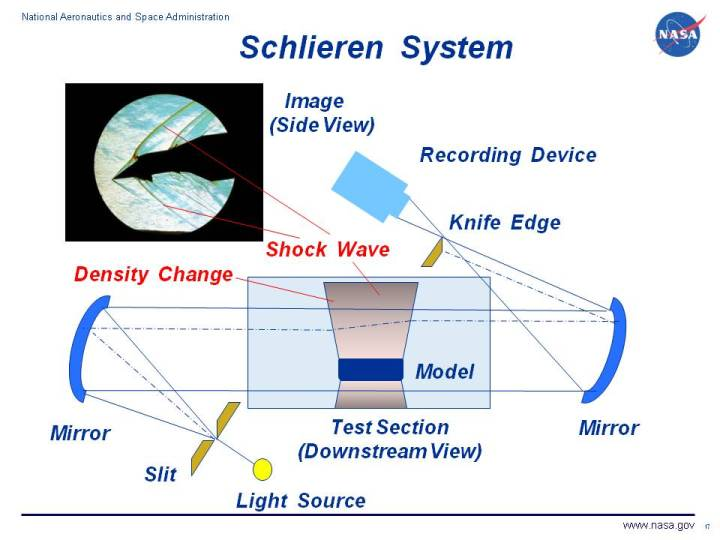
\includegraphics[scale = 0.75]{figures/schlieren_setup.jpg}
    \caption{Schematic of a z-type Schlieren system.\cite{Hall_2021}}
    \label{fig:schlieren_device}
\end{figure}


%%%%%%%%%%%%%%%%%%%%%%%
% Experimental Set-Up %
%%%%%%%%%%%%%%%%%%%%%%%


\section{Experimental Set-Up}

\noindent
This section details the lab setup and procedure used in the experiment.

\subsection{Apparatus}

The experiments are performed with an open circuit supersonic wind tunnel. A de Laval half-nozzle used to accelerate the flow to supersonic conditions is housed in the test section. A schematic of the wind tunnel's test section and the measurement instrumentation is provided in figure \ref{fig:chamber_setup}. The test section is a $25.4\si{mm} \text{ width} \times30\si{mm} \text{ height}$ rectangular prism with transparent plexiglass side windows. \newline

\noindent
The instrumentation consists of 11 static pressure taps (only the first 7 are used), and a horizontally traversable impact pressure probe (impact probe) with a range of motion between static taps 1 and 7; actuation is provided by two computer-controlled stepper motors. The impact probe is fixed vertically $5\si{mm}$ beneath the upper wall of the test section such that it measures along the equivalent centre line of a full de Laval nozzle. Static tap locations and nozzle geometry are presented in table \ref{tab:tap_locations}. The throat of the nozzle is located at static tap number 2; the test section levels off around static tap number 7. Therefore, the traversal range of the impact probe is sufficient to characterize the essential parts of the flow.\newline

\noindent
The static pressure taps and impact probe are connected using Tygon tubing to individual pressure transducers (Honeywell 142PC15A, 0-15 psi, unknown accuracy). The pressure transducers connect to the data acquisition computer using a DAQ card. The pressure transducers and impact probe stepper motor are controlled by a MATLAB program authored by P. McCarthy in October 2016.\newline

\noindent
It should be noted that during the experiment, the pressure transducer for static tap number 5 malfunctioned, providing inaccurate readings.\newline

\noindent
Shockwaves are visualized using a Z-type Schlieren imaging system similar to the illustration in figure \ref{fig:schlieren_device}. The reflecting elements consist of two 762 mm focal length parabolic mirrors mounted on an adjustable optical rail, illuminated by a lamp with a focusing lens to create a point source. The collimated light shines through the plexiglass windows of the test section, where it is reflected into a knife-edge at the focal point of the second mirror, where the remaining light shines onto a DSLR camera.

\begin{figure}[h]
    \centering
    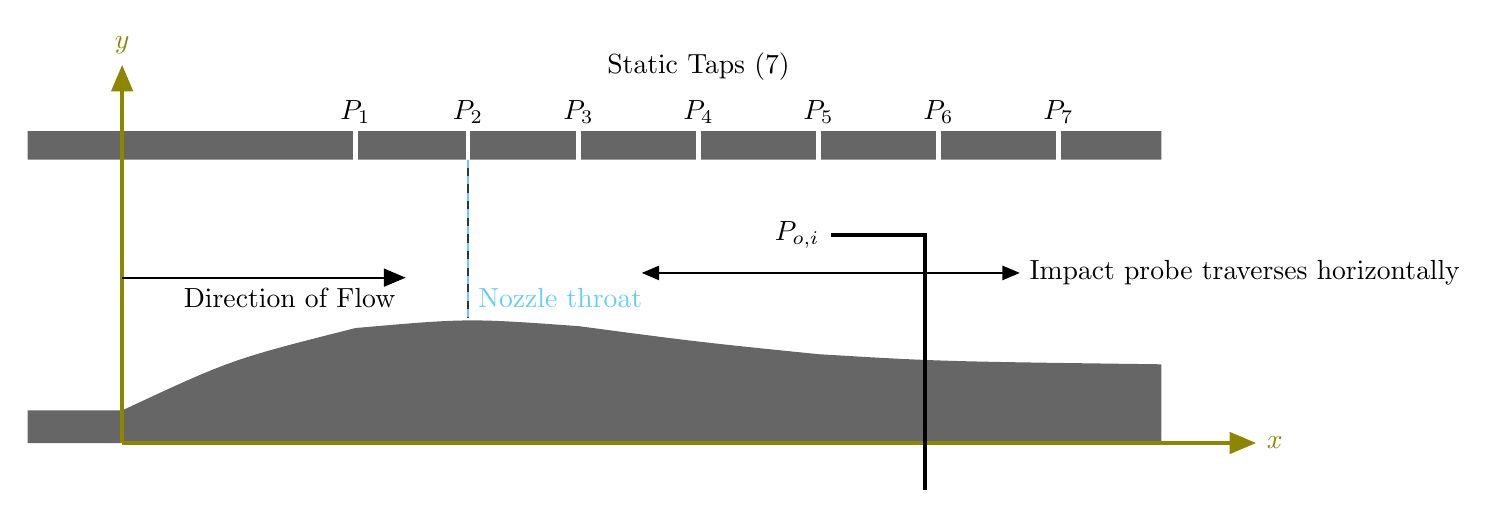
\begin{tikzpicture}[scale = 0.12]
    \fill[black!60] (0, 3.45) coordinate (A) .. controls (11.6, 8.86) .. (24.7, 12.17) .. controls (36.6, 13.21) .. (48.3, 12.37) .. controls (61, 10.69) .. (73.7, 9.40) .. controls (86.4, 8.64) .. (110, 8.33) -- (110, 0) -- (-10, 0) -- (-10, 3.45) -- cycle;
    \coordinate (B) at ($(A) +(0, 26.55)$);
    \fill[black!60] (B) -- +(110, 0) -- +(110, 3) -- +(-10, 3) -- +(-10, 0) -- cycle;
    \coordinate (P1) at ($(B) +(24.7, 0)$);
    \coordinate (P2) at ($(B) +(36.6, 0)$);
    \coordinate (P3) at ($(B) +(48.3, 0)$);
    \coordinate (P4) at ($(B) +(61.0, 0)$);
    \coordinate (P5) at ($(B) +(73.7, 0)$);
    \coordinate (P6) at ($(B) +(86.4, 0)$);
    \coordinate (P7) at ($(B) +(99.1, 0)$);
    \draw[white, ultra thick] (P1) -- +(0, 5) node[black]{$P_1$};
    \draw[white, ultra thick] (P2) -- +(0, 5) node[black]{$P_2$};
    \draw[white, ultra thick] (P3) -- +(0, 5) node[black]{$P_3$};
    \draw[white, ultra thick] (P4) -- +(0, 5) node[black]{$P_4$};
    \draw[white, ultra thick] (P5) -- +(0, 5) node[black]{$P_5$};
    \draw[white, ultra thick] (P6) -- +(0, 5) node[black]{$P_6$};
    \draw[white, ultra thick] (P7) -- +(0, 5) node[black]{$P_7$};
    \draw[olive, very thick, ->] (0, 0) -- (120, 0) node[right]{$x$};
    \draw[olive, very thick, ->] (0, 0) -- (0, 40) node[above]{$y$};
    \draw[thick, ->] (0, 17.5) -- +(30, 0) node[below left]{Direction of Flow};
    \draw[ultra thick, black] (85, -5) -- +(0, 27) -- +(-10, 27) coordinate (I) node[left]{$P_{o, i}$};
    \draw[<->, black] ($(I) +(-20, -4)$) -- +(40, 0) node[right]{Impact probe traverses horizontally};
    \draw (P4) node[above=25pt]{Static Taps (7)};
    \draw[black!80, thick] (P2) -- +(0, -16.79);
    \draw[dashed, cyan!60, thick] (P2) -- +(0, -16.79) node[above right]{Nozzle throat}; 
    \end{tikzpicture}
    \caption{Supersonic wind tunnel test section and de Laval half nozzle (to scale).}
    \label{fig:chamber_setup}
\end{figure}

\begin{figure}
    \centering
    \begin{subfigure}[b]{0.3\textwidth}
        \centering
        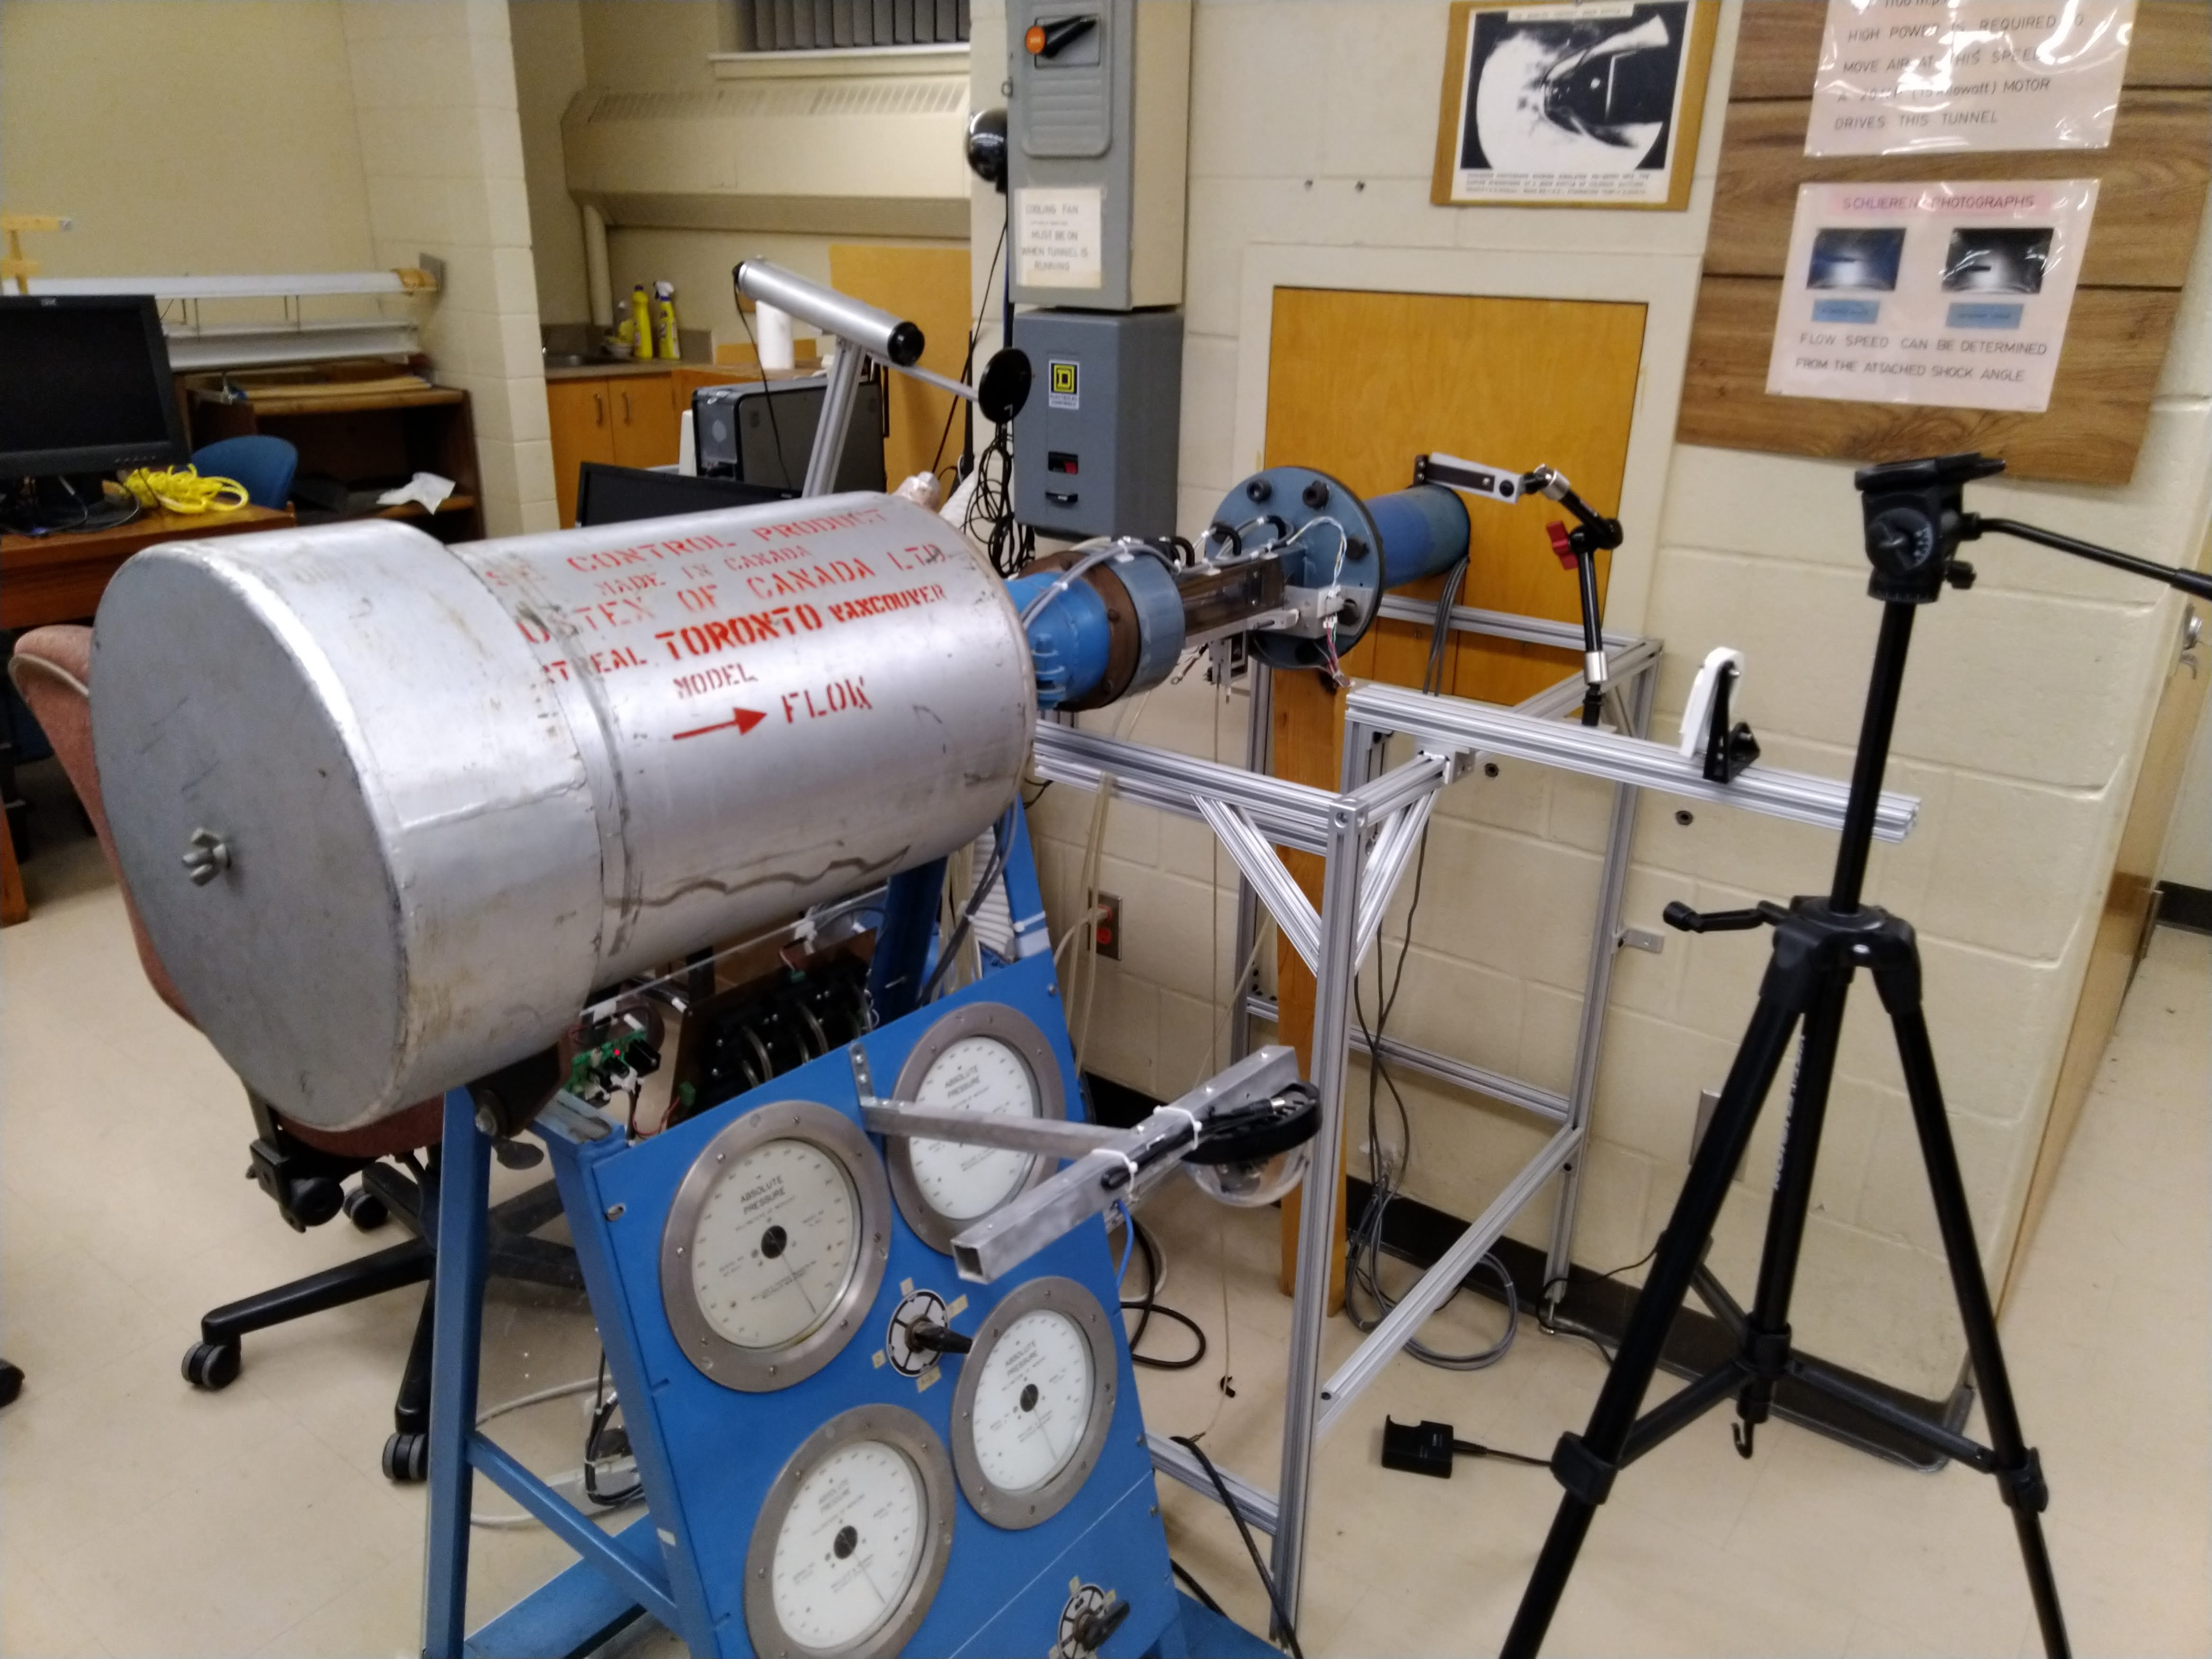
\includegraphics[width=\textwidth]{figures/Wide_Shot.jpg}
        \caption{The supersonic wind tunnel with the Schlieren imaging system set up around it.}
        \label{fig:setup_1}
    \end{subfigure}
    \hfill
    \begin{subfigure}[b]{0.3\textwidth}
        \centering
        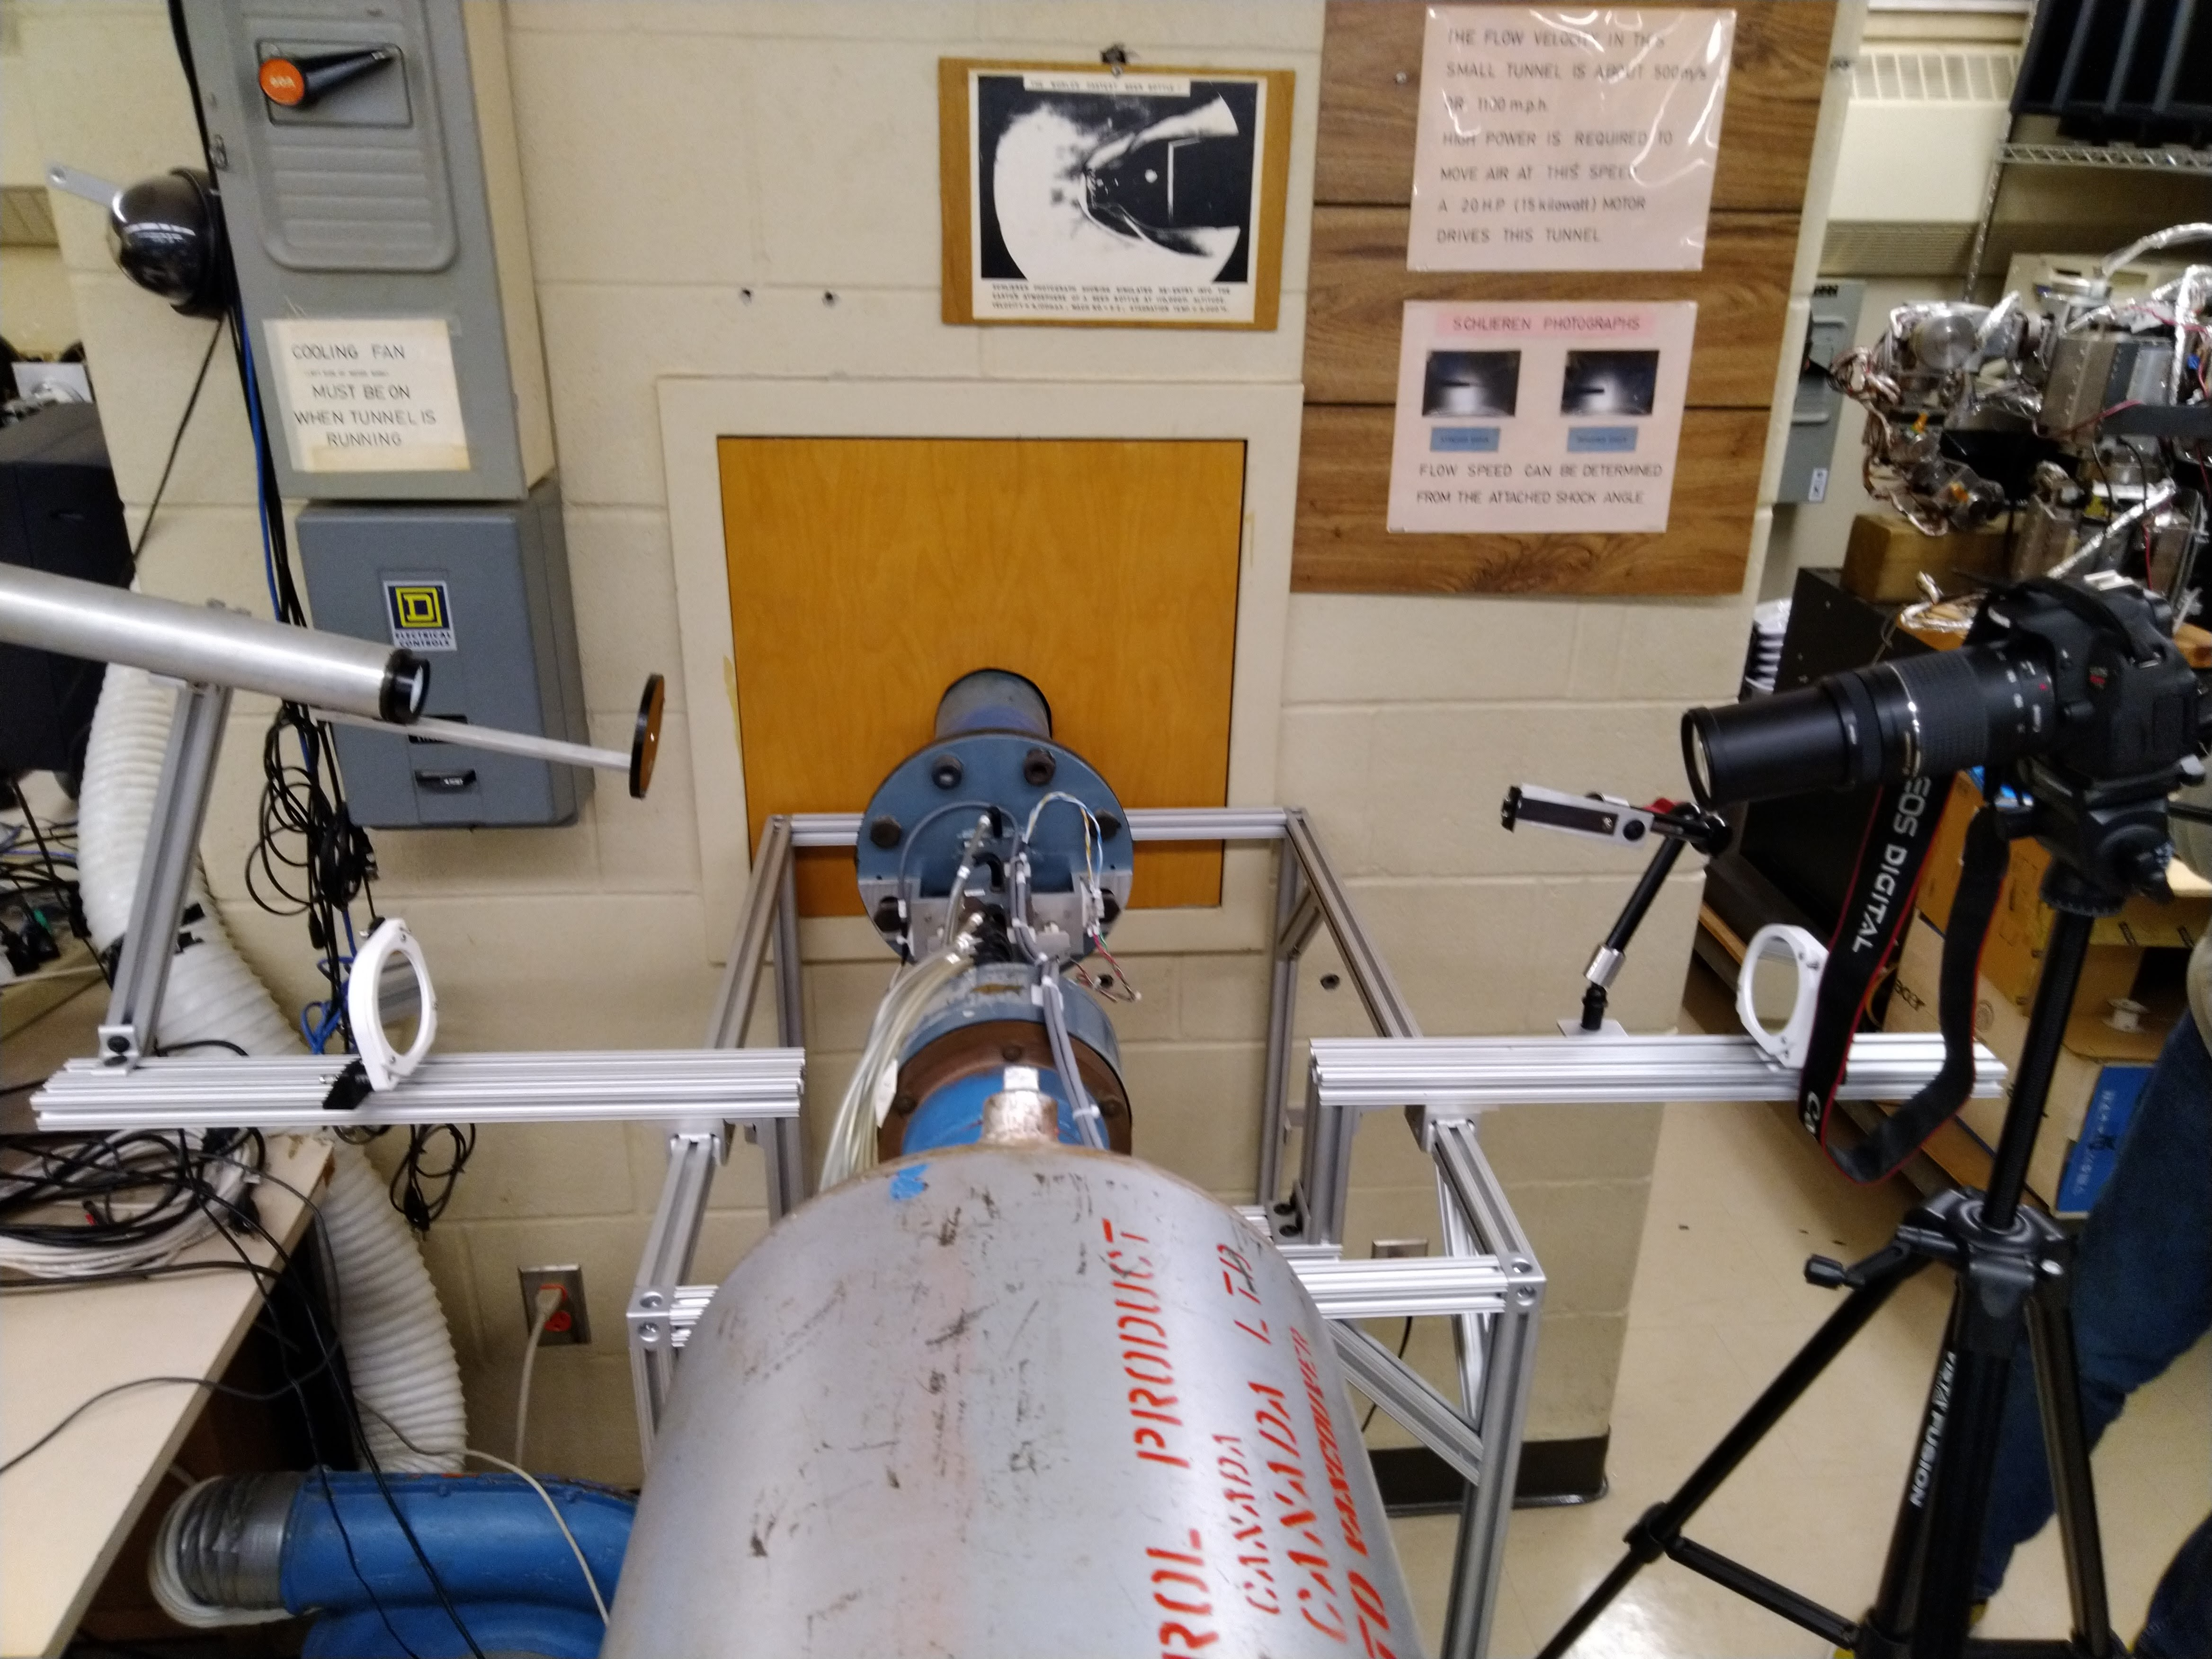
\includegraphics[width=\textwidth]{figures/Schlieren_System.jpg}
        \caption{The optical elements of the Schlieren system (light source, mirrors, knife edge, DSLR camera).}
        \label{fig:setup_2}
    \end{subfigure}
    \hfill
    \begin{subfigure}[b]{0.3\textwidth}
        \centering
        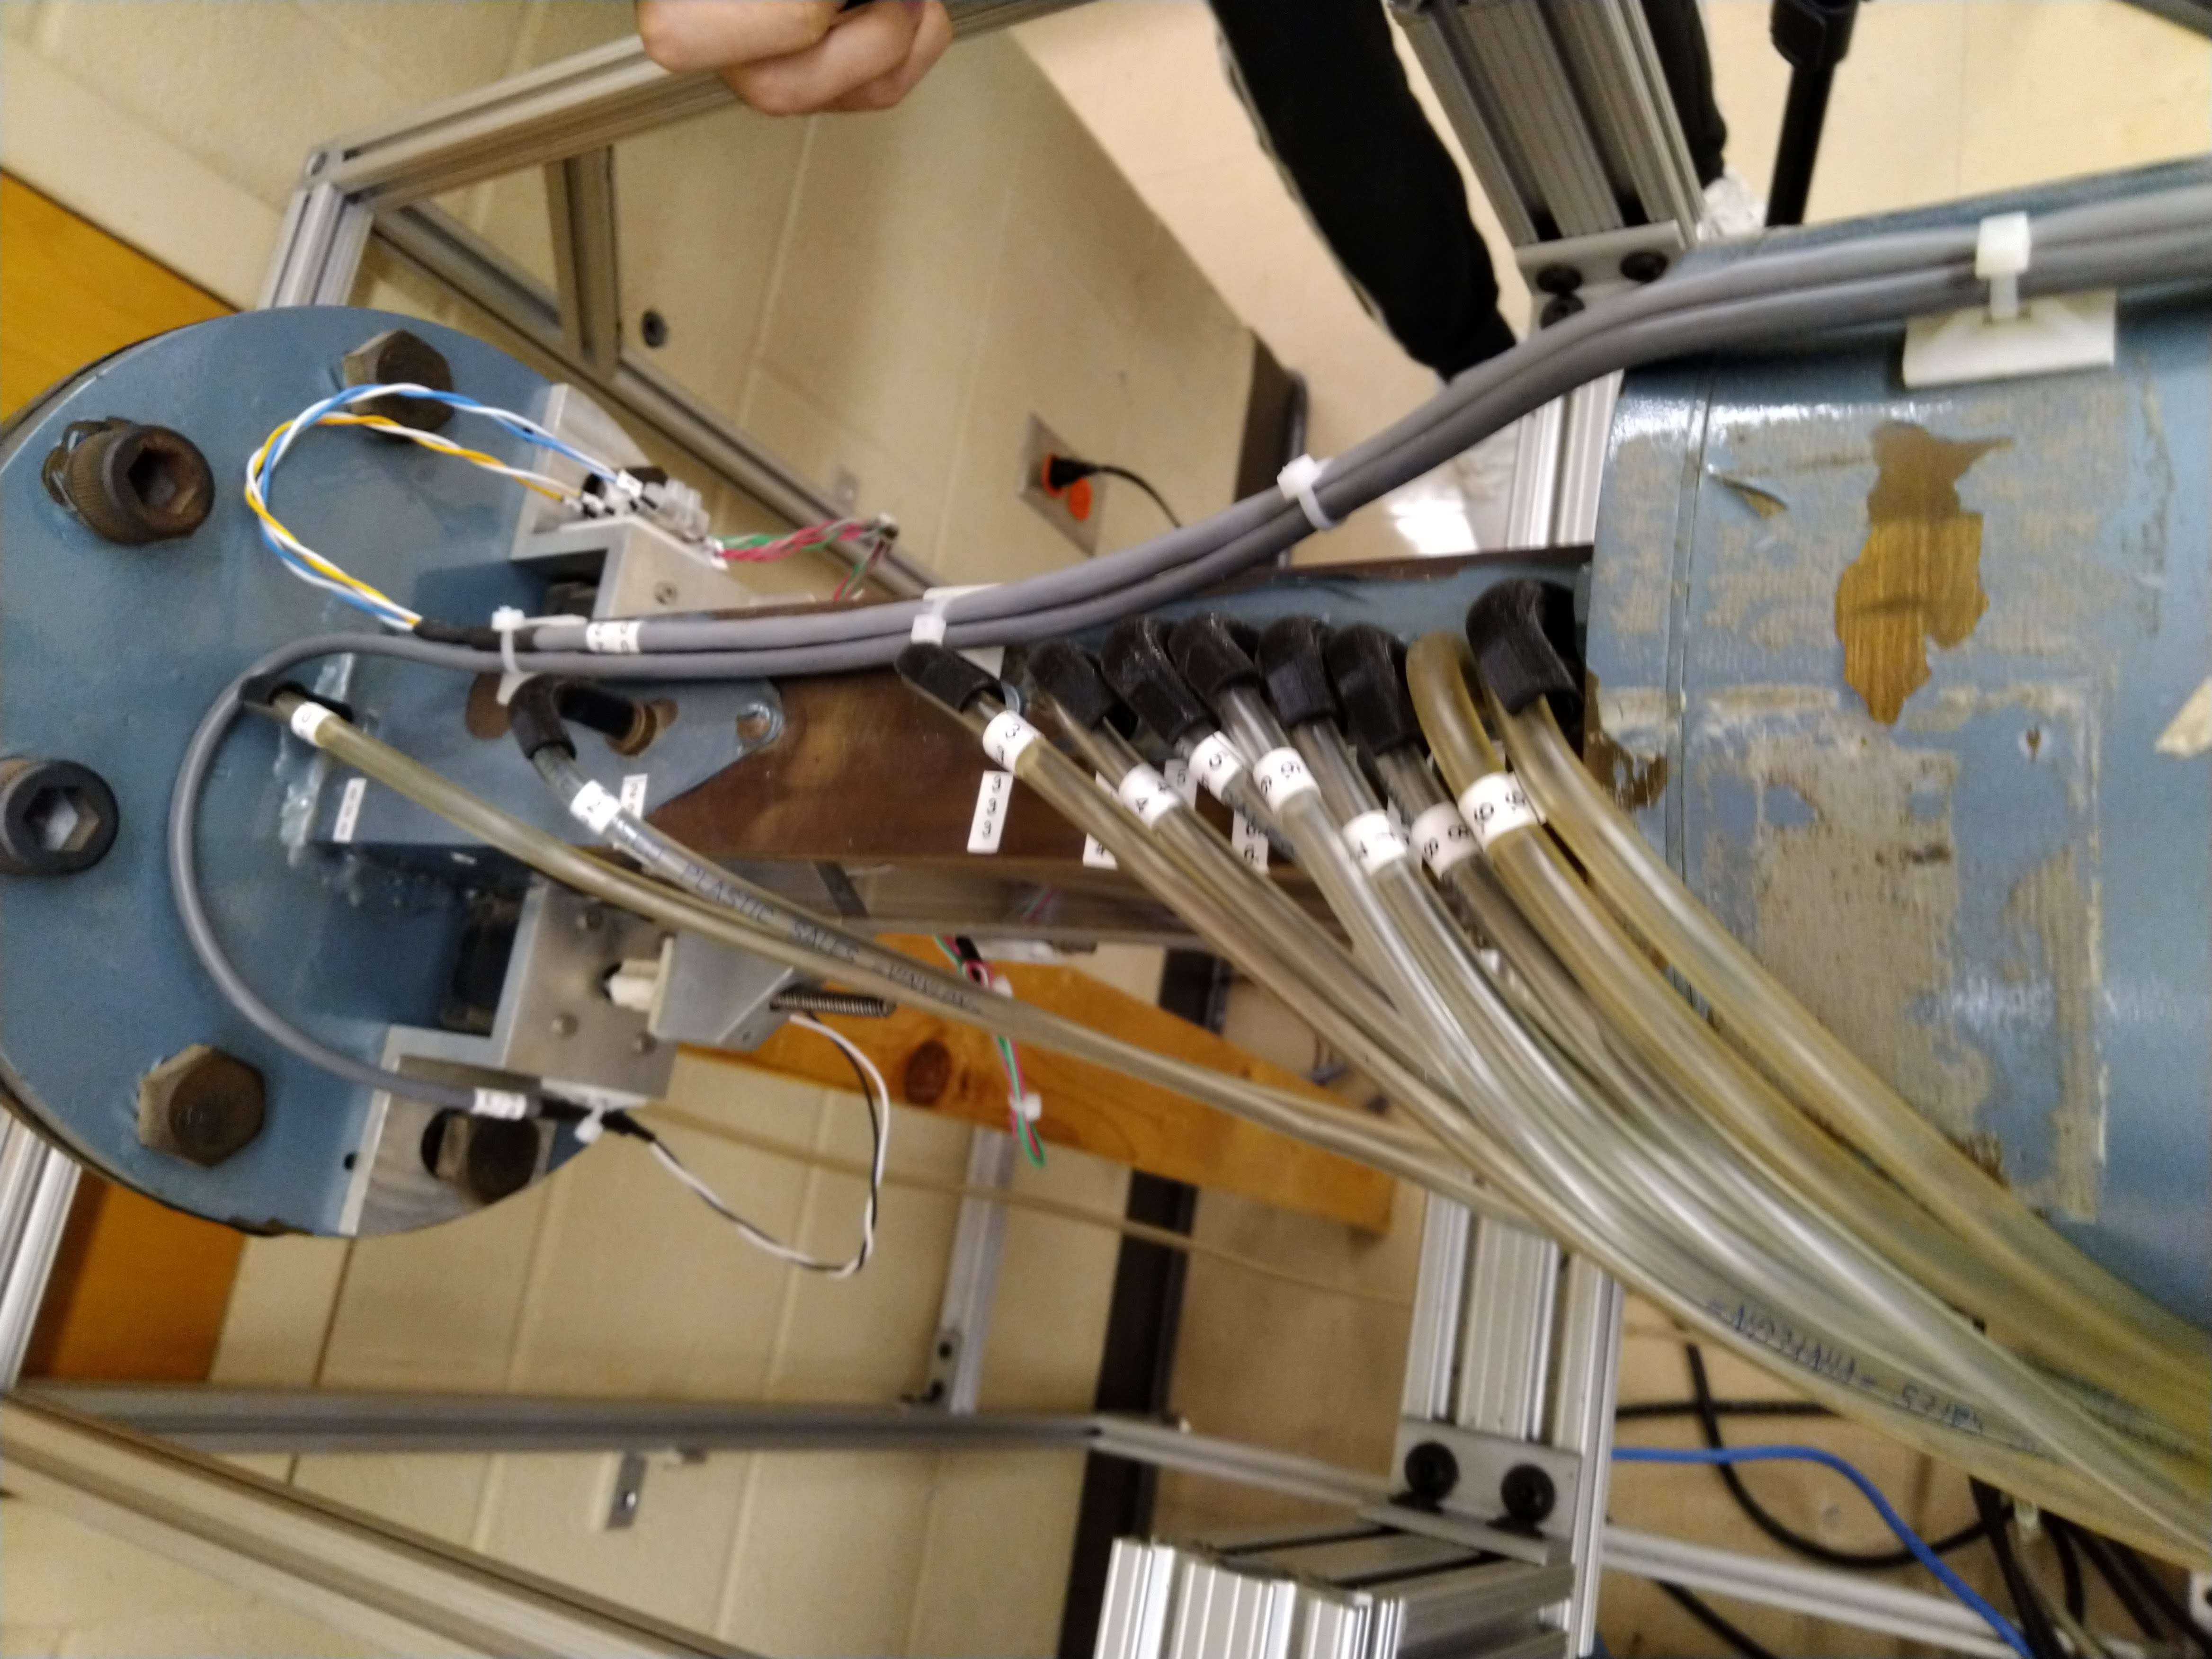
\includegraphics[width=\textwidth]{figures/Tygon_Tubes.jpg}
        \caption{Tygon tubes emerging from the static pressure taps in the test section.}
        \label{fig:setup_3}
    \end{subfigure}
    \caption{Pictures of the setup}
    \label{fig:setup_pictures}
\end{figure}

\begin{table}[h]
    \centering
    \begin{tabular}{p{3cm}p{1cm}p{1cm}p{1cm}p{1cm}p{1cm}p{1cm}p{1cm}}
        \toprule
        Tap Number & 1 & 2 & 3 & 4 & 5 & 6 & 7\\
        \midrule
        x (mm) & 24.7 & 36.6 & 48.3 & 61.0 & 73.7 & 86.4 & 99.1\\
        Nozzle Height (mm) & 12.17 & 13.21 & 12.37 & 10.69 & 9.40 & 8.64 & 8.33\\
        \bottomrule
    \end{tabular}
    \caption{Locations of the 7 pressure-taps and the nozzle geometry. $x$ is the distance from the start of the test section; nozzle height is measured from the bottom surface of the test section rear as seen in figure \ref{fig:chamber_setup}.}
    \label{tab:tap_locations}
\end{table}

\subsection{Procedure}\label{sec:procedure}

The procedure used for the acquisition of pressure measurements and shock visualization is as follows:

\begin{enumerate}

    \item With the wind tunnel off, offset measurements are collected for all pressure transducers using a MATLAB program.

    \item The wind tunnel is powered on and flow speed is adjusted using the manual valve such that all flow in the tunnel is subsonic. This is verified on the Schlieren imaging system by ensuring that there are no shocks in the test section.

    \item The static pressure distribution within the wind tunnel is measured from the 7 static pressure-taps. Data from all transducers are simultaneously collected using a MATLAB program on the data acquisition computer by taking a time series with an appropriate frequency and number of samples to provide $\pm 1 \%$ accuracy on each transducer.
    
    \item The total pressure at each of the 7 static pressure taps is measured by the traversing impact probe. A MATLAB program commands the stepper motor to move the impact probe to each of the 7 positions, the operator then takes pressure measurements after waiting for the flow to stabilize.
    
    \item The wind tunnel flow speed is increased using the manual valve such that all flow in the test section is supersonic. This is verified on the Schlieren imaging system by ensuring that there are no normal shocks in the test section, and confirming bow shocks are located in front of the impact probe. Steps 2 and 3 are then repeated for the supersonic case.
    
    \item Schlieren measurements are taken using the DSLR camera for the supersonic case.
    
    \item The wind tunnel flow speed is decreased to the transonic regime such that flow is partially subsonic and partially supersonic in the diverging section of the nozzle, and normal shocks are observed. Schlieren measurements are taken using the DSLR camera for the transonic case.

\end{enumerate}


%%%%%%%%%%%%%%%%%%%%%%%%%%
% Results and Discussion %
%%%%%%%%%%%%%%%%%%%%%%%%%%


\section{Results and Discussion}

This section details the analysis of pressure and Mach number distributions for the subsonic and supersonic regimes. Additionally, the theoretical and experimental approaches are compared.

\subsection{Subsonic Regime}

% what was being measured...
% what was done with the data...
% Describe the data...
% What are the implications of the data...
% What are cross-connections in the data...
\subsubsection{Theoretical and Experimental Mach Number Distribution:}
\label{sec:sup_mach_comp}
% Introduce the Mach number distributions, how was the theoretical calculated, how was the experimental calculated, how do the two results match? What does this imply?
The subsonic regime is explored using the Mach number distribution of the wind tunnel test section. Both theoretical and experimental approaches are used. The theoretical approach employs methods detailed in section \ref{sec:thy_Mach_calc} which assume an incompressible, inviscid and isentropic flow. The incompressibility and inviscid assumptions are valid due to the near-constant total pressure experienced in the test section (as seen in figure \ref{fig:subsonic_pressure}). Additionally, the lack of shocks validates the isentropic assumption, for there is no significant heat dissipation due to shocks. The experimental approach applies the isentropic relation directly to the pressure data and only assumes an isentropic flow.\newline

\noindent
The theoretical and experimental Mach number distributions are shown in figure \ref{fig:subsonic_Mach}. In both cases, the Mach number increases for taps 1 and 2 where the nozzle converges; the Mach number then decreases for the remaining taps where the nozzle diverges. This behaviour is in line with the expectations of subsonic flow in a Venturi. The discrepancies between the theoretical and experimental distributions are small and may be the result of unsteady flow and viscous forces. Conventionally, compressibility effects are considered negligible for $M < 0.3$. However, the peak Mach number observed in the experiment of approximately 0.42 exceeds this threshold, implying some (albeit small) compressibility effects contributing to the discrepancy.\newline

\noindent
No shocks were observed during the subsonic flow using the Schlieren technique, meaning that the isentropic assumption holds well for this case.\newline

\noindent
\subsubsection{Theoretical and Experimental Pressure Distribution:}
The subsonic Mach regime is also explored through theoretical and experimental analysis of the static pressure distribution along the length of the test section. The theoretical approach determines the pressure distribution using incompressible continuity and Bernoulli's equation. The comparison of the two approaches can be seen in figure \ref{fig:subsonic_pressure_comp}.\newline

\noindent
The theoretical and experimental pressure distributions coincide well except at higher tap numbers (ignoring tap number 5 because of the faulty transducer). Here, the deviation from theoretical predictions is possibly due to the inviscid assumption of the theoretical model. In reality, the viscous effects in the narrow test section would cause energy dissipation and lower pressure readings than the theoretical case (as seen in figure \ref{fig:subsonic_pressure_comp}); the deviations also grow near the end of the test section as the effects of energy dissipation are compounded.

\begin{figure}[h]
    \centering
    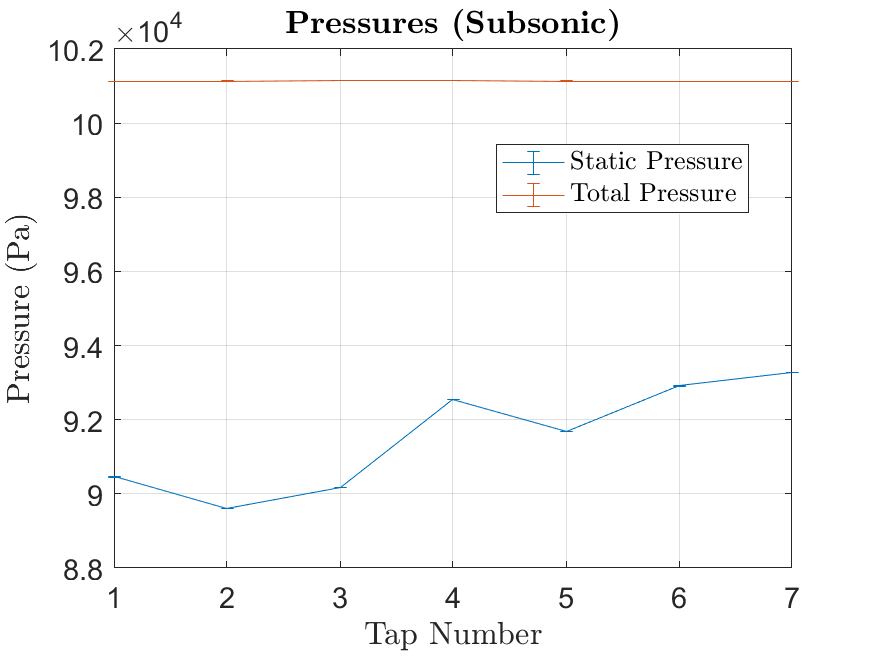
\includegraphics[width=0.5\textwidth]{figures/subsonic_pressure_distributions.png}
    \caption{Subsonic static and total pressure distributions.}
    \label{fig:subsonic_pressure}
\end{figure}

\begin{figure}[h]
    \centering
    \begin{subfigure}{0.49\textwidth}
    \includegraphics[width=\textwidth]{figures/subsonic_Mach_distributions.png}
    \caption{Subsonic Mach number distributions.}
    \label{fig:subsonic_Mach}
    \end{subfigure}
    \hfill
    \begin{subfigure}{0.49\textwidth}
    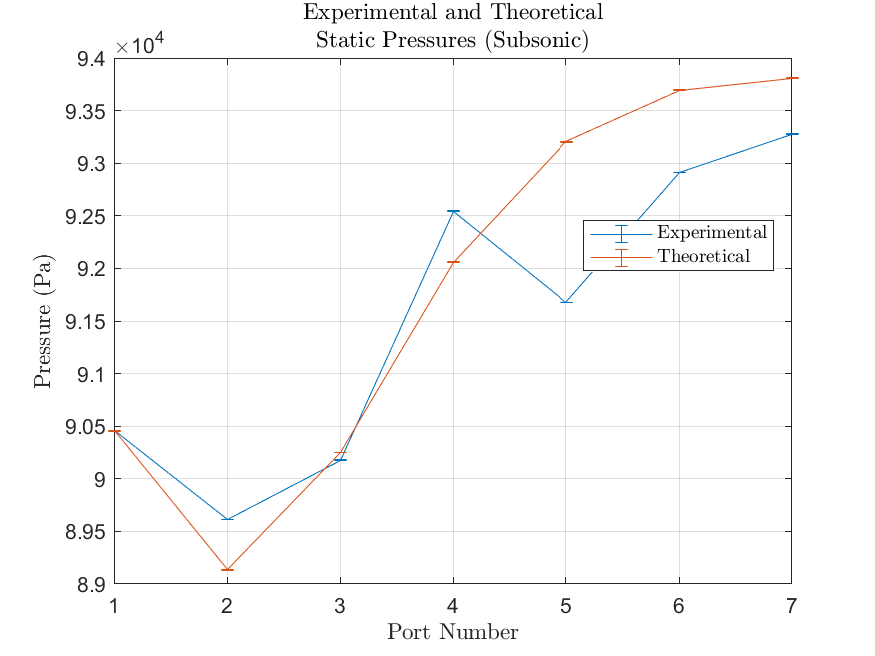
\includegraphics[width=\textwidth]{figures/subsonic_pressure_distribution_exp_vs_thy.png}
    \caption{Subsonic static pressure distributions.}
    \label{fig:subsonic_pressure_comp}
    \end{subfigure}
    \caption{Subsonic Mach and pressure distributions for experimental and theoretical results.}
    \label{fig:subsonic_comp}
\end{figure}

\subsection{Supersonic Regime}

% \noindent
% Comparison between theoretical prediction and experimental data about Mach number and pressure distribution are plotted in figure \ref{fig:supersonic_comp}.\newline

\subsubsection{Theoretical and Experimental Mach Number Distribution:}

\noindent
The supersonic Mach regime is explored using the Mach number distribution of the test section with theoretical and experimental approaches. The theoretical approach utilizes the methods discussed in section \ref{sec:thy_Mach_calc}, primarily using the area-Mach number relation (equation \ref{eq:background_1}); for each tap location, the cross-sectional area is determined and the area-Mach number relation is numerically solved for the supersonic Mach number, $M$. Such methods assume only isentropic flow. For the experimental case, equation \ref{eq:supersonic_Mach_relation} is numerically solved for $M$ given the total and static pressure measurements of each pressure tap. The comparison between the two approaches is seen in figure \ref{fig:supersonic_Mach}.\newline

\noindent
The Mach number behaviour for the theoretical and experimental cases behave as expected. In the converging portion of the test section (tap 1), the flow is subsonic and becomes sonic at the throat (tap 2). The diverging portion of the test section (taps 3 - 7) is associated with accelerating supersonic flow. With this in mind, there are deviations between the theoretical and experimental distributions, most notably for taps 6 and 7 (tap 5 is faulty). The primary cause for such deviation is the isentropic assumption of the theoretical model. The presence of the impact probe in the supersonic flow results in bow shocks. The shock waves are sources of heat release, which in turn creates energy loss, thereby violating the isentropic assumption of the theoretical model. The significance of violation of the isentropic assumption can be seen in figure \ref{fig:supersonic_pressure} where the total pressure decrease signifies energy losses due to shocks. Additionally, viscous effects in the small test section result in energy losses, causing a lower Mach number to be achieved than expected; this claim is supported by figure \ref{fig:supersonic_Mach}. These effects are most prominent at the end of the test section end due to compounding effects and higher flow velocity.

\begin{figure}[h]
    \centering
    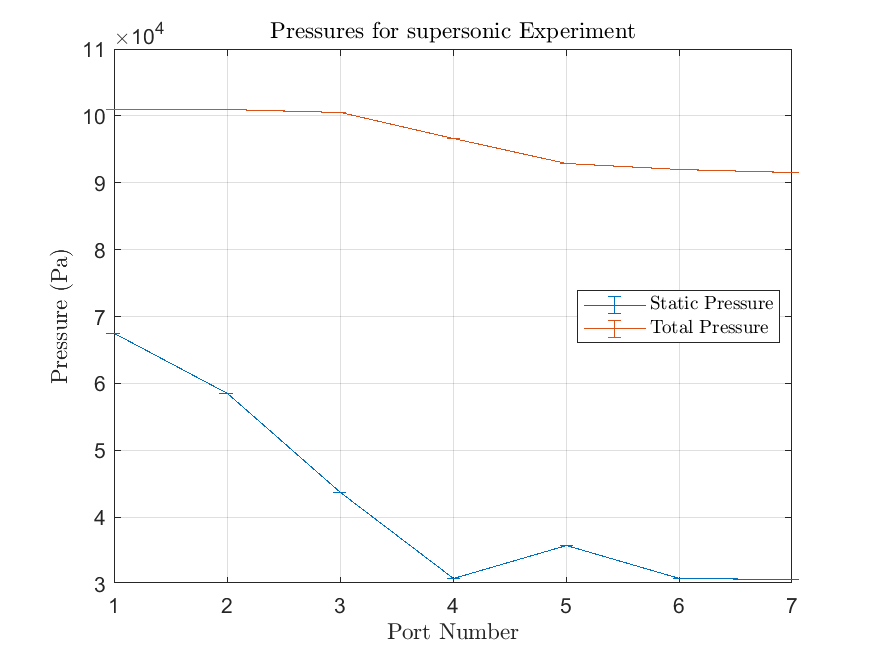
\includegraphics[width  = 0.49\textwidth]{figures/supersonic_pressure_distributions.png}
    \caption{Supersonic static and total pressure distributions.}
    \label{fig:supersonic_pressure}
\end{figure}

\begin{figure}[h]
    \centering
    \begin{subfigure}{0.49\textwidth}
    \includegraphics[width=\textwidth]{figures/supersonic_Mach_distributions.png}
    \caption{Supersonic Mach number distributions.}
    \label{fig:supersonic_Mach}
    \end{subfigure}
    \hfill
    \begin{subfigure}{0.49\textwidth}
    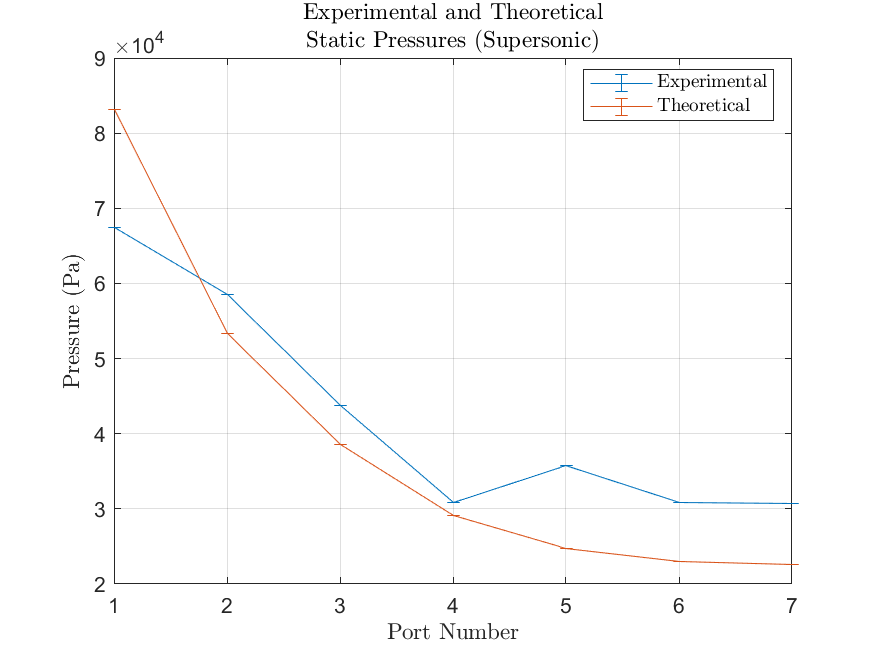
\includegraphics[width=\textwidth]{figures/supersonic_pressure_distribution_exp_vs_thy.png}
    \caption{Supersonic static pressure distributions.}
    \label{fig:supersonic_pressure_comp}
    \end{subfigure}
    \caption{Supersonic pressure and Mach number distributions comparison for experimental and theoretical results.}
    \label{fig:supersonic_comp}
\end{figure}

\subsubsection{Theoretical and Experimental Pressure Distribution:}

The supersonic regime is also explored through the theoretical and experimental analysis of the pressure distribution along the length of the test section. Using the methods in section \ref{sec:theoretical_pressure_cals}, the theoretical pressure distribution is calculated from the theoretical Mach number distribution, assuming an isentropic flow. The experimental pressure distribution is determined directly from measurements made through pressure transducers. A comparison between the two approaches can be seen in figure \ref{fig:supersonic_pressure_comp}.\\

\noindent
The distributions behaviour aligns closely to expectations. The pressure monotonically decreases over the length of the test section, which relates to the necessary density changes in the flow to ensure the direction of flow and conservation of mass. Comparing the two distributions, there exist only small deviations between theoretical and experimental values. The theoretical data is calculated from the theoretical Mach number distribution inherits error due to the isentropic assumption and viscous effects in the test section.

\subsection{Schlieren Images}

\subsubsection{Supersonic Case:}

Bow shocks are observed locally when supersonic flow meets the front of the impact probe which stagnates the supersonic flow. The flow field downstream of the bow shock and impact probe remains supersonic. This is illustrated schematically in figure \ref{fig:supersonic_shocks}.\\

\begin{figure}[h]
    \centering
    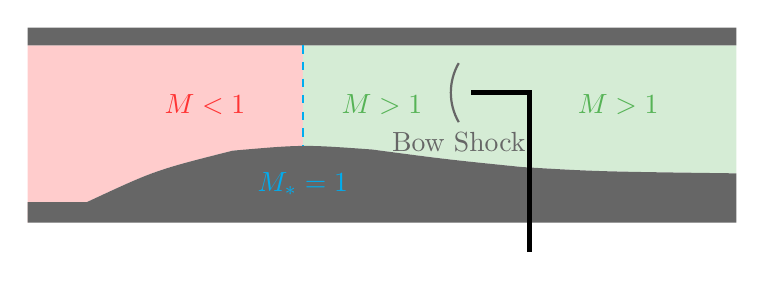
\begin{tikzpicture}[scale = 0.075]
    % SUBSONIC REGION
    \fill[red!20]  (0, 3.45) .. controls (11.6, 8.86) .. (24.7, 12.17) -- (36.6, 13) -- (36.6, 30) -- (-10, 30) -- (-10, 0) -- cycle;
    % SUPERSONIC REGION
    \fill[green!20]  (36.6, 13) -- (48.3, 12.37) .. controls (61, 10.69) .. (73.7, 9.40) .. controls (86.4, 8.64) .. (110, 8.33) -- (110, 30) -- (36.6, 30) -- cycle;
    \fill[black!60] (0, 3.45) coordinate (A) .. controls (11.6, 8.86) .. (24.7, 12.17) .. controls (36.6, 13.21) .. (48.3, 12.37) .. controls (61, 10.69) .. (73.7, 9.40) .. controls (86.4, 8.64) .. (110, 8.33) -- (110, 0) -- (-10, 0) -- (-10, 3.45) -- cycle;
    \coordinate (B) at ($(A) +(0, 26.55)$);
    \fill[black!60] (B) -- +(110, 0) -- +(110, 3) -- +(-10, 3) -- +(-10, 0) -- cycle;
    \draw[ultra thick] (75, -5) -- +(0, 27) -- +(-10, 27) coordinate (BOW);
    \draw[thick, black!60] (BOW) +(-2, 5) arc (150:210:10) node [below]{Bow Shock};
    \draw[thick, dashed, cyan] (36.6, 30) -- (36.6, 13) node[below=6 pt]{$M_* = 1$};
    \draw[red!80] (20, 20) node {$M < 1$};
    \draw[green!80] (50, 20) node {$M > 1$};
    \draw[green!80] (90, 20) node {$M > 1$};
    \end{tikzpicture}
    \caption{Flow conditions for supersonic case.}
    \label{fig:supersonic_shocks}
\end{figure}

\noindent
Figure \ref{fig:schlieren_1} shows a bow shock observed under fully supersonic conditions. Additional oblique shock waves are visible due to reflection off the top and bottom surfaces of the test section. The bow shock was observed to be steady and did not oscillate.

\subsubsection{Transonic Case:}

Normal shocks are observed throughout the entire height of the test section whenever there is a supersonic-to-subsonic transition within the flow field. As a result, the flow downstream of a normal shock is subsonic. This is illustrated schematically in figure \ref{fig:transonic_shocks}.

\begin{figure}[h]
    \centering
    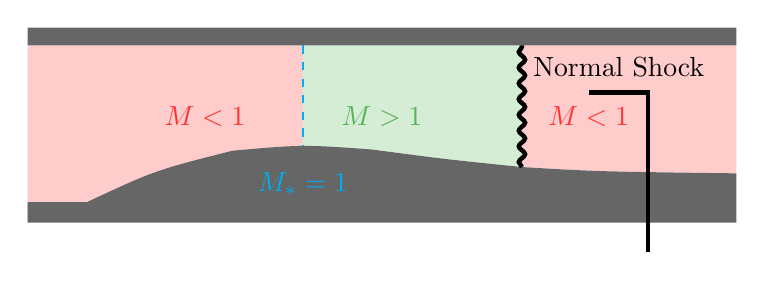
\begin{tikzpicture}[scale = 0.075]
    % SUBSONIC REGION 1
    \fill[red!20]  (0, 3.45) .. controls (11.6, 8.86) .. (24.7, 12.17) -- (36.6, 13) -- (36.6, 30) -- (-10, 30) -- (-10, 0) -- cycle;
    % SUPERSONIC REGION
    \fill[green!20]  (36.6, 13) -- (48.3, 12.37) .. controls (61, 10.69) .. (73.7, 9.40) -- (73.7, 30) -- (36.6, 30) -- cycle;
    % SUBSONIC REGION 2
    \fill[red!20]  (73.7, 9.40) .. controls (86.4, 8.64) .. (110, 8.33) -- (110, 30) -- (73.7, 30) -- cycle;
    \fill[black!60] (0, 3.45) coordinate (A) .. controls (11.6, 8.86) .. (24.7, 12.17) .. controls (36.6, 13.21) .. (48.3, 12.37) .. controls (61, 10.69) .. (73.7, 9.40) .. controls (86.4, 8.64) .. (110, 8.33) -- (110, 0) -- (-10, 0) -- (-10, 3.45) -- cycle;
    \coordinate (B) at ($(A) +(0, 26.55)$);
    \fill[black!60] (B) -- +(110, 0) -- +(110, 3) -- +(-10, 3) -- +(-10, 0) -- cycle;
    \draw[ultra thick] (95, -5) -- +(0, 27) -- +(-10, 27) coordinate (BOW);
    % THROAT AND MACH
    \draw[thick, dashed, cyan] (36.6, 30) -- (36.6, 13) node[below=6 pt]{$M_* = 1$};
    \draw[red!80] (20, 18) node {$M < 1$};
    \draw[green!80] (50, 18) node {$M > 1$};
    \draw[red!80] (85, 18) node {$M < 1$};
    % NORMAL SHOCKS
    \tikzset{decoration={snake,amplitude=.4mm,segment length=2mm,
                       post length=0mm,pre length=0mm}}
    \draw[decorate, ultra thick] (73.7, 9.40) -- (73.7, 30) node[below right] {Normal Shock};
    \end{tikzpicture}
    \caption{Flow conditions for transonic case.}
    \label{fig:transonic_shocks}
\end{figure}

\noindent
Normal shocks occur when the flow is not entirely supersonic in the diverging portion of the test section. Deceleration of supersonic flow in the diverging section is possible in a real wind tunnel because of non-ideal losses which are not accounted for in the isentropic assumptions made earlier.\newline

\noindent
Figure \ref{fig:schlieren_2} shows a normal shock and the absence of a bow shock on the impact probe demonstrating subsonic conditions downstream of the shock. The observed shock was turbulent, hence the apparent softness of the image compared to the bow shock. Additionally, figures \ref{fig:schlieren_3} and \ref{fig:schlieren_4} show a bow shock forming on the impact probe when placed upstream of the normal shock demonstrating the supersonic-subsonic transition.

\begin{figure}[h]
    \centering
    \begin{subfigure}{0.49\textwidth}
    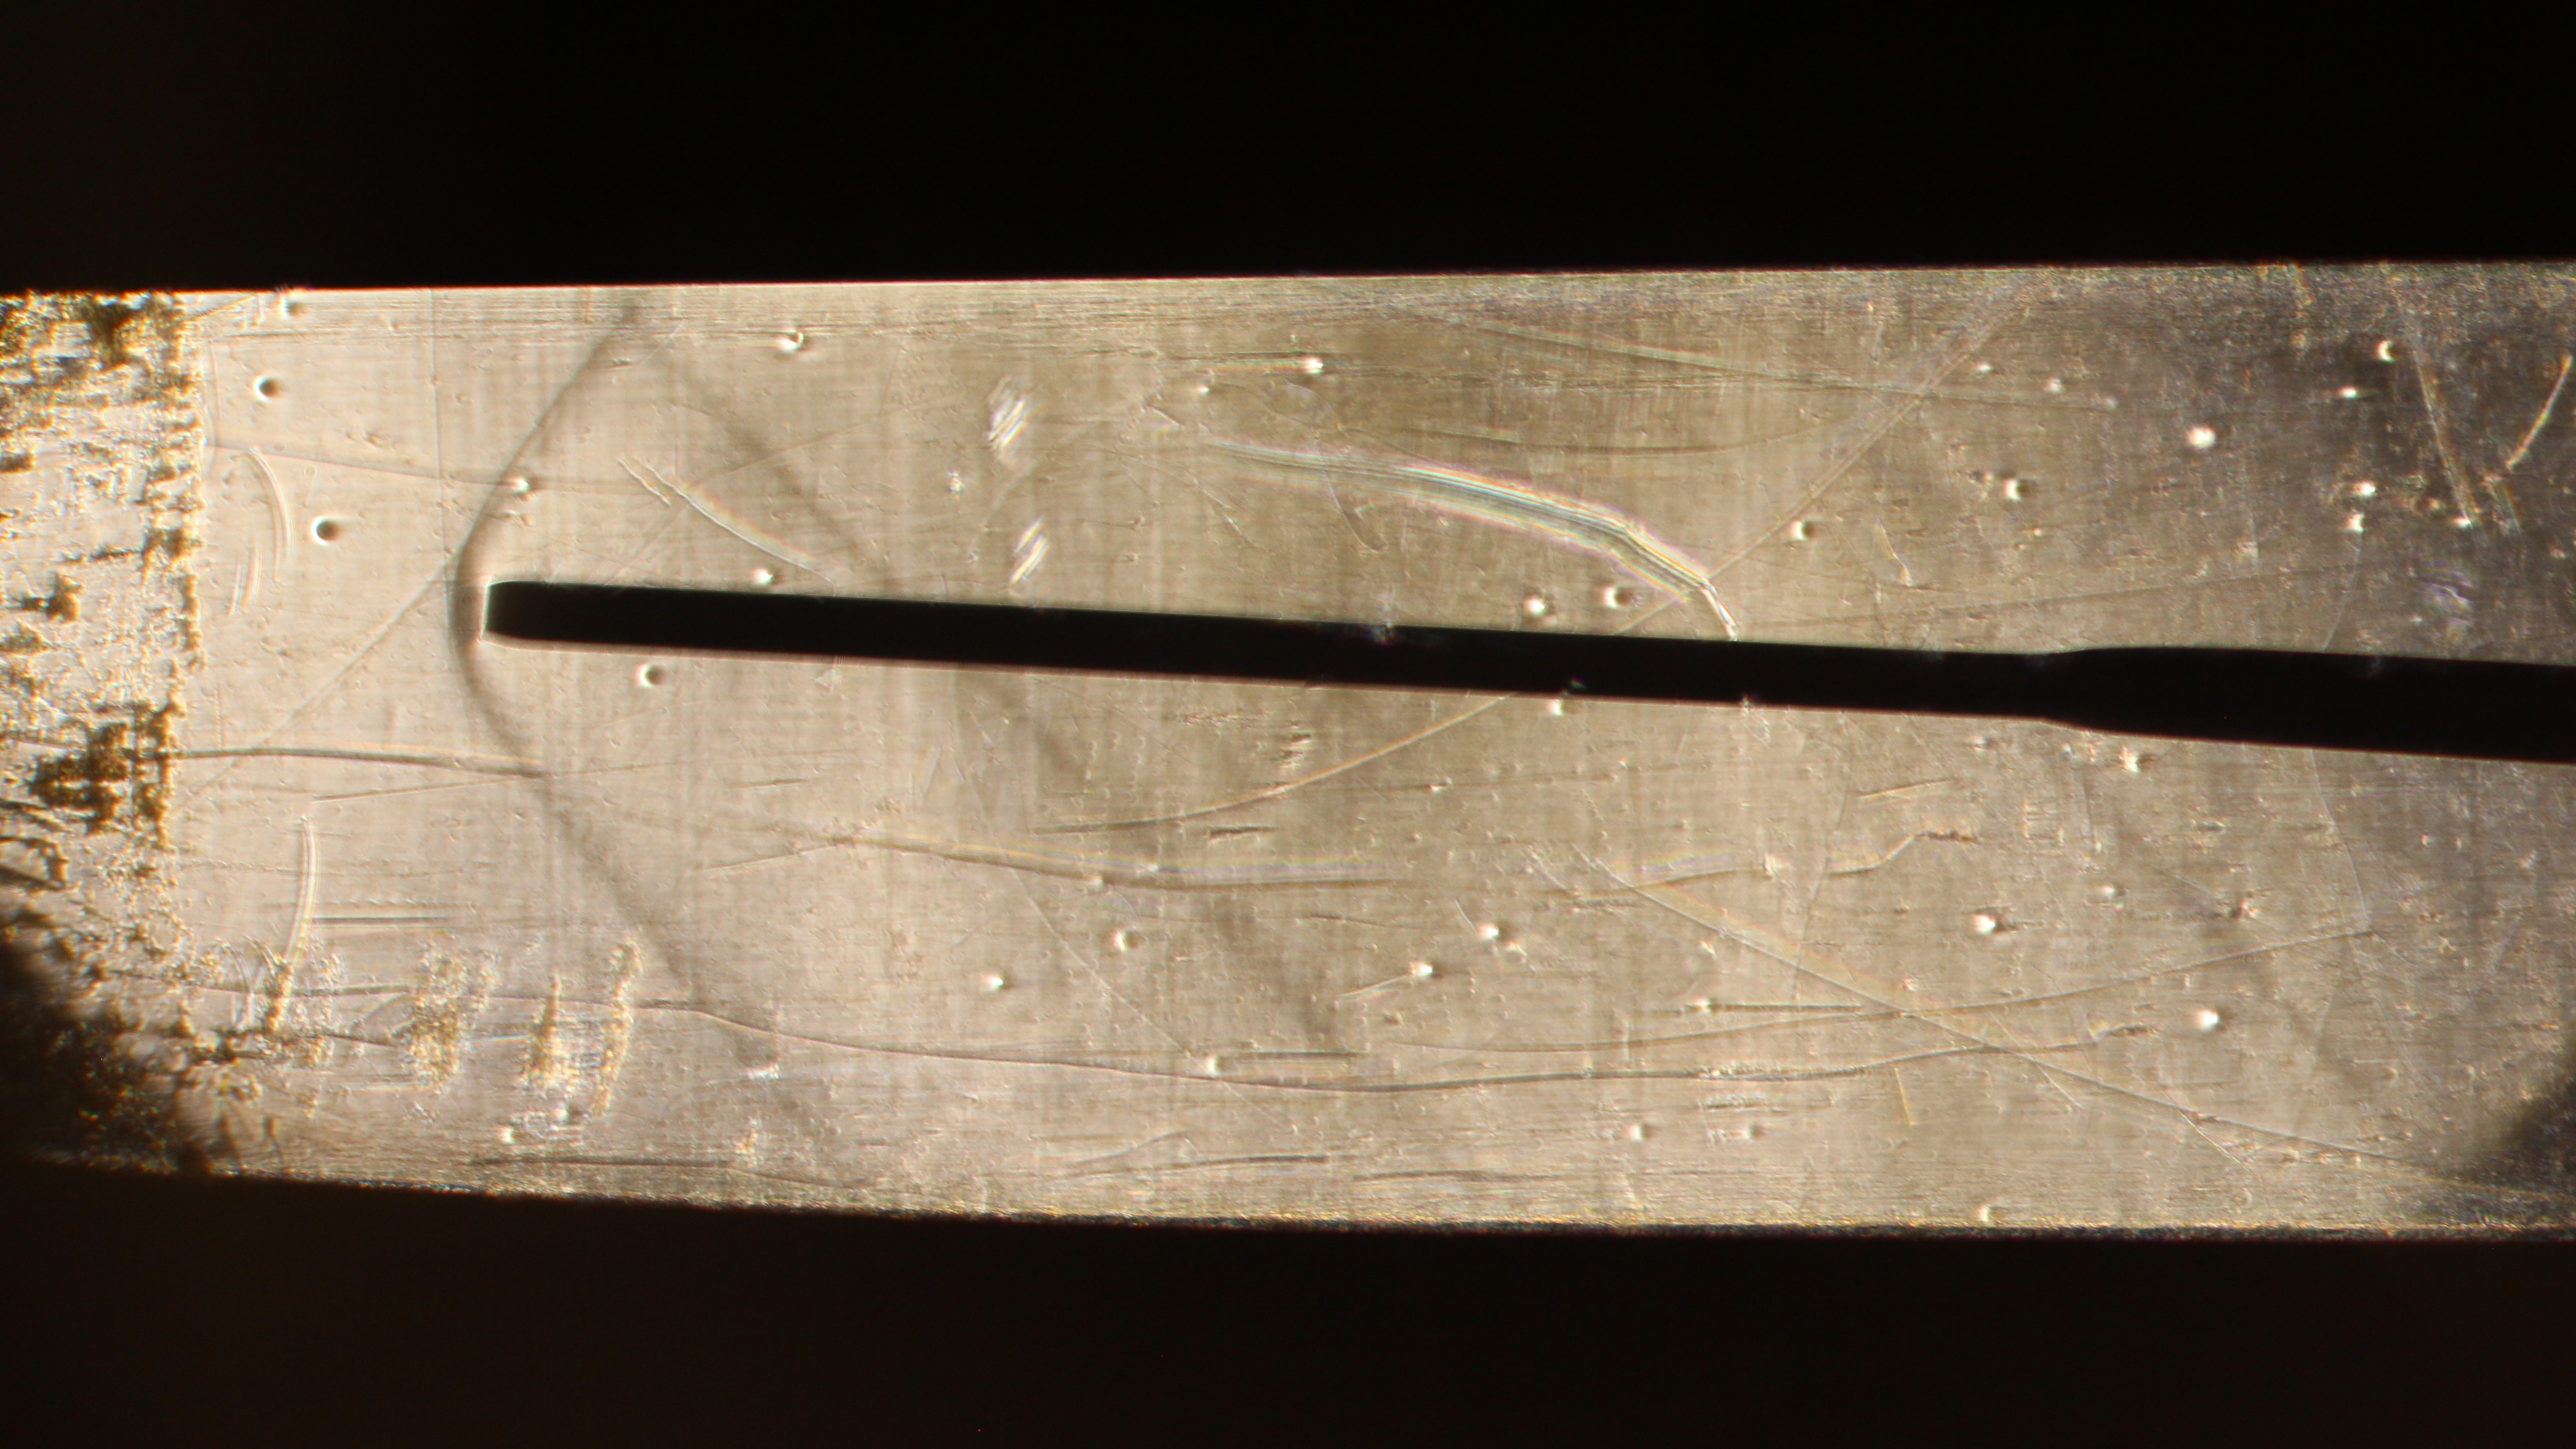
\includegraphics[width=\textwidth]{figures/IMG_3994.JPG}
    \caption{Bow shock under fully supersonic flow conditions.}
    \label{fig:schlieren_1}
    \end{subfigure}
    \hfill
    \begin{subfigure}{0.49\textwidth}
    \includegraphics[width=\textwidth]{figures/IMG_4002.JPG}
    \caption{Normal shock forming through the entire height of the test section due to supersonic-subsonic transition.}
    \label{fig:schlieren_2}
    \end{subfigure}
    \begin{subfigure}{0.49\textwidth}
    \includegraphics[width=\textwidth]{figures/IMG_4022.JPG}
    \caption{Bow shock in front of the impact probe in supersonic part of flow field, along with a normal shock.}
    \label{fig:schlieren_3}
    \end{subfigure}
    \hfill
    \begin{subfigure}{0.49\textwidth}
    \includegraphics[width=\textwidth]{figures/IMG_4025.JPG}
    \caption{Interactions between bow shock and normal shock.}
    \label{fig:schlieren_4}
    \end{subfigure}
    \caption{Shock wave visualization using the Schlieren technique.}
    \label{fig:schlieren_imaging}
\end{figure}

%%%%%%%%%%%%%%%%%%%%
% Sources of Error %
%%%%%%%%%%%%%%%%%%%%


\section{Sources of Error}
\label{sec:source_of_error}

\subsection{Quantifiable Sources of Error}

The only quantifiable source of error is the precision uncertainty associated with the pressure time series data of each pressure tap. The error was obtained using equation \ref{eq:...} where $\sigma$ is the standard deviation of the time series and $N$ is the number of samples collected. Sampling time was adjusted to exceed the integral timescale of the data such that all collected samples are assumed independent. The pressure data and associated uncertainties are tabulated in table \ref{tab:pressure_data}.

\begin{equation}
    P = 1.96 \frac{\sigma}{\sqrt{N}}
    \label{eq:...}
\end{equation}

\subsection{Non-Quantifiable Sources of Error}

Non-quantifiable sources of error include errors associated with the pressure transducer, the effects of the unsteady flow, and the long travel distance of air to the transducer which results in the damping of short duration pressure transients.\newline

\noindent
\textbf{Pressure Transducer} The bias and precision error of the pressure transducer are not provided by the manufacturer. We are unable to determine their error, and it was assumed to be zero.\newline

\noindent
\textbf{Unsteady Flow} The nature of the unsteady flow in the wind tunnel introduces error into our calculation, as static and total pressure measurements are not taken simultaneously. \newline

\noindent
\textbf{Transient Effect of Pressure Tubes}  The pressure changes need to travel down the length of the tube to be recorded by the pressure transducer; damping effects are present during transportation. \newline

\noindent
Furthermore, the traversal of the impact probe is only controllable to within a finite position, and the tip of the impact probe was observed to oscillate vertically from interactions with the flow field; all of this to say that the total pressure measurements do not exactly correspond to the static pressure measurements.


%%%%%%%%%%%%%%
% Conclusion %
%%%%%%%%%%%%%%


\section{Conclusion}

The pressure and Mach number distributions were determined for the de Laval half-nozzle in a supersonic wind tunnel. Total and static pressure measurements were taken for both the subsonic and supersonic flow regimes and were compared to theoretical predictions. There was good agreement between the theoretical and experimental pressure distributions for both regimes; although, deviations near the end of the test section grew and are most likely due to the inviscid assumption of the theoretical model which does not reflect the losses in the experiment. The Mach number distributions for the subsonic case had deviations suspected to result from the incompressible assumption of the theoretical prediction not capturing compressibility effects. For the supersonic Mach number distributions, the error is a result of the invalid isentropic assumption from the presence of shocks. The inviscid assumption of the theoretical Mach number calculations are also believed to contribute to the observed deviations of the Mach number distributions.\newline

\noindent
Localized bow shocks were observed in the supersonic flow case, and normal shocks were observed in the transonic flow case using the z-type Schlieren imaging system. The shocks were observed under conditions consistent with theoretical predictions for their formation. The presence of shocks in the supersonic flow provides a clear indication of losses which renders the isentropic assumption invalid in the supersonic case. \newline

\noindent
It is hypothesized that the significant deviations in theoretical and experimental pressure and Mach number distributions are a result of viscous effects. To validate this hypothesis, future iterations of the experiment should include viscous effects in the theoretical predictions. The resulting distributions should then be cross-referenced with the inviscid theoretical prediction and experimental case.
Other improvements can also be made in future iterations of the experiment. Multiple measurements at each pressure tap can be performed to decrease bias error associated with noisy measurements and unsteady flow. Moreover, bias errors of instrumentation in the experiment can be determined from references or by other experiments to better estimate the bias error of the measurement instruments. \newline


\noindent
In summary, this experiment was successful in comparing the theoretical predictions to experimental methods in Mach number and pressure distributions of different flow regimes, as well as visualizing shock waves in transonic and supersonic flow. \newline




%%%%%%%%%%%%%%%%
% Bibliography %
%%%%%%%%%%%%%%%%


\newpage
\bibliographystyle{IEEEtran}
\bibliography{biblio}


%%%%%%%%%%%%
% Appendix %
%%%%%%%%%%%%


\newpage
\appendix
\noindent
{\LARGE \textbf{Appendix}}

\section{Pressure Measurements}

Refer to table \ref{tab:pressure_data} for the static and total pressure measurements for the subsonic and supersonic cases.

\begin{table}[h]
    \centering
    \begin{tabular}{p{2cm}p{3.5cm}p{3.5cm}p{3.5cm}p{3.5cm}}
        \toprule
        Measure & Subsonic Static ($\si{Pa}$) & Subsonic Total ($\si{Pa}$) & Supersonic Static ($\si{Pa}$) & Supersonic Total ($\si{Pa}$) \\
        \midrule
        Tap 1 & $090460.0 \pm 2.0$ & $101130.0 \pm 2.3$ & $067420.0 \pm 3.2$ & $101010.0 \pm 2.7$ \\
        Tap 2 & $089610.0 \pm 2.6$ & $101140.0 \pm 2.4$ & $058550.0 \pm 3.6$ & $101010.0 \pm 2.9$ \\
        Tap 3 & $090180.0 \pm 2.7$ & $101140.0 \pm 2.3$ & $043700.0 \pm 3.4$ & $100520.0 \pm 3.0$ \\
        Tap 4 & $092550.0 \pm 1.7$ & $101140.0 \pm 2.4$ & $030830.0 \pm 2.0$ & $096570.0 \pm 3.4$ \\
        Tap 5 & $091680.0 \pm 1.8$ & $101140.0 \pm 2.4$ & $035750.0 \pm 2.4$ & $092850.0 \pm 3.6$ \\
        Tap 6 & $092910.0 \pm 1.5$ & $101120.0 \pm 2.4$ & $030850.0 \pm 1.7$ & $092020.0 \pm 3.2$ \\
        Tap 7 & $093280.0 \pm 1.9$ & $101120.0 \pm 2.1$ & $030700.0 \pm 8.6$ & $091570.0 \pm 3.4$ \\
        \bottomrule
    \end{tabular}
    \caption{Static and total pressure measurements for the subsonic and supersonic trials.}
    \label{tab:pressure_data}
\end{table}

\section{Uncertainty Propagation}

This appendix details the error propagation formulas used in the error analysis within this lab. It is useful to note the error propagation formula for $y(x_1,.....,x_M)$ is as seen in equation \ref{eq:error_prop}

\begin{align}
    \delta y &= \sqrt{\sum_{i=1}^M \left( \diffp{y}{{x_i}} \delta x_i\right)^2}
    \label{eq:error_prop}
\end{align}

\subsection{(Subsonic Theoretical) Velocity via Bernoulli}

Flow velocity at tap 1, obtained from the static pressure at tap 1 and the total pressure, was used to determine flow conditions at all other taps in the subsonic case. Assume $\rho$ is known perfectly.

\begin{align*}
    P_1 + \frac{1}{2}\rho U_1^2 &= P_o\\
    U_1 &= \sqrt{\frac{2(P_o - P_1)}{\rho}}\\
    \delta U_1 &= \frac{1}{U_1 \rho}\sqrt{\delta P_o^2 + \delta P_1^2}
\end{align*}

\subsection{(Subsonic Theoretical) Velocity via Continuity}

Flow velocity at tap $i$ for $i = {2, ..., 7}$, obtained from area ratio and flow velocity at tap 1.
\begin{align*}
    U_i &= \frac{A_1}{A_i} U_1\\
    \delta U_i &= \frac{A_1}{A_i} U_1
\end{align*}

\subsection{(Subsonic Theoretical) Static Pressure}

Static pressure at tap $i$ for $i = {2, ..., 7}$, obtained from Bernoulli.

\begin{align*}
    P_i &= P_o - \frac{1}{2} \rho U_i^2\\
    \delta P_i &= \sqrt{\left(\diffp{{P_i}}{{P_o}} \delta P_o\right)^2 + \left(\diffp{{P_i}}{{U_i}} \delta U_i \right)^2}\\
    \delta P_i &= \sqrt{\left(\delta P_o\right)^2 + \left(\rho U_i \delta U_i \right)^2}
\end{align*}

\subsection{(Subsonic Theoretical) Local Speed of Sound}

The local speed of sound at each tap is obtained using the Ideal Gas Law.

\begin{align*}
    a_i &= \sqrt{\frac{\gamma P_i}{\rho}}\\
    \delta a_i &= \frac{\gamma}{2 a_i \rho} \delta P_i
\end{align*}

\subsection{(Subsonic Theoretical) Mach Number}
\begin{align*}
    M_i &= \frac{U_i}{a_i}\\
    \delta M_i &= \sqrt{(\tfrac{1}{a_i} \delta U_i)^2 + (\tfrac{U_i}{a_i^2} \delta a_i)^2}
\end{align*}

\subsection{(Subsonic Experimental) Mach Number}

\begin{align*}
    M &= \sqrt{\frac{2}{\gamma - 1}}\left[\left(\frac{P_o}{P}\right)^\frac{\gamma - 1}{\gamma} - 1\right]^{\frac{1}{2}} \\
    \delta M &= \sqrt{\left(\frac{\partial M}{\partial P_o}\delta P_o\right)^2 + \left(\frac{\partial M}{\partial P}\delta P\right)^2}\;\text{where}\;
    \frac{\partial M}{\partial P_o} = \frac{P^\frac{1 - \gamma}{2\gamma}P_o^{- \frac{1}{-\gamma}}(\gamma - 1)^\frac{1}{2}}{2^\frac{1}{2}\gamma\left(P_o^\frac{\gamma - 1}{\gamma} - P^\frac{\gamma - 1}{\gamma}\right)^\frac{1}{2}}\;\text{,}\;\frac{\partial M}{\partial P} -\frac{P_o^\frac{\gamma - 1}{\gamma}P^\frac{1 - 3\gamma}{2\gamma}(\gamma - 1)^\frac{1}{2}}{2^\frac{1}{2}\gamma\left(P_o^\frac{\gamma - 1}{\gamma} - P^\frac{\gamma - 1}{\gamma}\right)^\frac{1}{2}}
\end{align*}

\subsection{(Supersonic Theoretical) Mach Number}
The theoretical Mach Number is calculated using \verb 'fzero()' function in MATLAB numerically using equation \ref{eq:background_1}. The numerical method has a tolerance threshold, and we take the absolute difference between the true area ratio $\frac{A}{A_*}$ and the area ratio calculated using computed Mach number, $\frac{\Tilde{A}}{A_*}.$

$$\delta M = \left| \frac{A}{A_*} - \frac{\Tilde{A}}{A_*} \right|$$

\subsection{(Supersonic Theoretical) Static Pressure}

\begin{align*}
    P &= P_o\cdot K, K \equiv \left(\frac{\gamma + 1}{2}M^2\right)^{\frac{-\gamma}{\gamma - 1}}\\
    \delta P &= \sqrt{\left(\frac{\partial P}{\partial P_o} \delta P_o\right)^2 + \left(\frac{\partial P}{\partial K} \delta K\right)^2}\\
    \frac{\partial P}{\partial K} \delta K &= \frac{\partial P}{\partial M} \delta M \\
    \frac{\partial P}{\partial P_o} &= K\\
    \frac{\partial P}{\partial M} &= -\frac{2\,M\,\gamma \,{\left(\frac{\gamma }{2}-\frac{1}{2}\right)}}{{{\left({\left(\frac{\gamma }{2}-\frac{1}{2}\right)}\,M^2 +1\right)}}^{\frac{\gamma }{\gamma -1}+1} \,{\left(\gamma -1\right)}} \equiv S\\
    \Rightarrow \delta P &= \sqrt{\left(K \delta P_o\right)^2 + \left(S\delta K\right)^2}
\end{align*}

\subsection{(Supersonic Experimental) Mach Number}

\begin{align*}
    \frac{P_o}{P} &= \left(\frac{\gamma + 1}{2}M^2\right)^{\frac{\gamma}{\gamma - 1}}\left(\frac{2\gamma}{\gamma + 1}M^2 - \frac{\gamma - 1}{\gamma + 1}\right)^{-\frac{1}{\gamma - 1}} \\
    &\Rightarrow g(P_o, P) = f(M) \\
    &\Rightarrow \delta f = \sqrt{\left(\frac{\partial g}{\partial P_o}\delta P_o\right)^2 + \left(\frac{\partial g}{\partial P}\delta P\right)^2}\;\text{but}\;\delta f = \frac{\partial f}{\partial M} \delta M \\
    &\Rightarrow \delta M = \left(\frac{\partial f}{\partial M}\right)^{-1}\sqrt{\left(\frac{\partial g}{\partial P_o}\delta P_o\right)^2 + \left(\frac{\partial g}{\partial P}\delta P\right)^2}
\end{align*}
where
\begin{align*}
    \frac{\partial f}{\partial M} &= \frac{\gamma (\gamma + 1) M}{\gamma - 1}\left(\frac{\gamma + 1}{2}M^2\right)^\frac{1}{\gamma - 1}\left(\frac{2\gamma}{\gamma + 1}M^2 - \frac{\gamma - 1}{\gamma + 1}\right)^{-\frac{1}{\gamma - 1}} + \\ & \ \ \frac{4\gamma M}{(\gamma + 1)(\gamma - 1)}\left(\frac{\gamma + 1}{2}M^2\right)^\frac{1}{\gamma - 1}\left(\frac{2\gamma}{\gamma + 1}M^2 - \frac{\gamma - 1}{\gamma + 1}\right)^{\frac{-\gamma}{\gamma - 1}} \\
    \frac{\partial g}{\partial P} &= -\frac{P_o}{P^2} \\
    \frac{\partial g}{\partial P_o} &= -\frac{1}{P}
\end{align*}

\newpage
\section{MATLAB and Python Code}

\subsection{Main Code}

\inputminted{matlab}{code/main.m}

\subsection{Raw Data Manipulation}
\inputminted{matlab}{code/get_pressures.m}
\inputminted{matlab}{code/get_uncertainties.m}

\subsection{Subsonic Experimental Analysis}

\inputminted{matlab}{code/subsonic_experimental.m}
\inputminted{matlab}{code/subsonic_experimental_err.m}


\subsection{Subsonic Theoretical Analysis}

\inputminted{matlab}{code/subsonic_theoretical.m}

\subsection{Supersonic Experimental Analysis}

\inputminted{matlab}{code/supersonic_experimental.m}
\inputminted{matlab}{code/supersonic_experimental_err.m}

\subsection{Supersonic Theoretical Analysis}

\inputminted{matlab}{code/supersonic_theoretical.m}

\subsection{Generation of Area-Mach Relationship Plot}
\inputminted{matlab}{code/area_mach_relation_plot.m}

\end{document}